\chapter{Introduction}

The swarm project is set out to build permissionless storage and communication infrastructure for tomorrow's self-sovereign digital society. Such a system needs to come with a browser interface, so that it can act as a decentralised alternative to today's world wide web. From a developer's perspective, swarm is best seen as public infrastructure that powers real-time interactive web applications familiar from the web 2.0 era. It provides low-level API to primitives that serve as building blocks of complex applications as well as the basis for the tools and libraries for a swarm-based web3 development stack.

This chapter details the design and architecture of the system and captures the result of nearly 5 years of work. In accordance with the principles laid out in \ref{sec:design-principles}, we put an emphasis on modular design, and conceive of swarm as having clearly separable layers, each dependent on the previous one: (1) a peer-to-peer network protocol to serve as underlay transport, (2) an overlay network with protocols powering a distributed immutable storage of chunks (fix-sized data blocks),  (3) a component for higher-level data access defining APIs for the base-layer features, and (4) an application layer potentially defining the standards, capturing best practices for more elaborate use-cases. We consider both (1) and (4) outside the scope of this book.

We will present the narrative with the incentivisation discussed in separate chapters giving rise to the following structure:
The architecture of the swarm overlay network is discussed in \ref{sec:network} and is complemented by \ref{sec:incentivisation} describing the system of economic incentives which makes swarm self-sustained. In \ref{sec:high-level-data-access}, we introduce the algorithms and conventions that allow swarm to map data concepts relating to storage such as file, collection, key-value store, access control onto the chunk layer as well as describes a user interface to the storage component. \ref{sec:messaging} defines communication primitives such as direct message, communication channel, resource updates, subscription and notifications in terms of chunks and offers a user interface for the communication component. Finally,  \ref{sec:persistence} is dedicated to techniques that, on various levels, contribute to data persistence and enables swarm to serve as a permanent data store. 

\chapter{Network}\label{sec:network}

This chapter offers a narrative how the swarm overlay network (\ref{sec:overlay-addressing}) is built on top of a peer-to-peer network protocol (\ref{sec:underlay-transport}). Nodes running the swarm client can discover each other, bootstrap and maintain a certain overlay topology (\ref{sec:bootstrapping}), that allows for efficient routing (\ref{sec:kademlia-routing}). In \ref{sec:kademlia-storage}, we describe how such a network can serve as a scalable distributed storage solution for chunks \ref{sec:chunks} and present the logic behind the protocols for retrieval/download (\ref{sec:retrieval}) and syncing/upload (\ref{sec:syncing}).

\section{Topology and routing}\label{sec:topology-routing}



\subsection{Underlay transport}\label{sec:underlay-transport} 

Swarm is a network operated by its users. Each node in the network is supposed to run a client complying with the protocol specifications. On the lowest level, the nodes in the network connect using a peer to peer network protocol as their transport layer. This is called the \gloss{underlay network}. 
In its overall design, swarm is agnostic of the particular underlay transport used as long as it satisfies the following requirements.

\begin{enumerate}
    \item \emph{addressing} Nodes are identified by their underlay address
    \item \emph{dialling} Nodes can initiate a direct connection to a peer by dialing them on their underlay address
    \item \emph{listening} Nodes can listen to other peers dialing them and can accept incoming connections
    \item \emph{live connection} A node connection establishes a channel of communication which is kept alive until explicit disconnection, so that the existence of a connection means the remote peer is online and accepting messages
    \item \emph{channel security} 
    the channel provides identity verification and implements encrypted and authenticated transport resisting man in the middle attacks
    \item \emph{protocol multiplexing} 
    The underlay network service can accommodate several protocols running on the same connection. Peers communicate the protocols (with name and versions) they implement and the underlay service identifies compatible protocols and starts up peer connections on each matched protocol. 
    \item \emph{delivery guarantees}
    Protocol messages are guaranteed to be delivered, i.e., delivery failures due to network problems result in direct error response. 
    Order of delivery of messages within each protocol is guaranteed. 
    Ideally the underlay protocol provides prioritisation. 
    If protocol multiplexing is over the same transport channel, this most likely implies framing so that long messages do not block higher priority messages.
    \item \emph{serialisation} 
    The protocol message construction supports arbitrary data structure serialisation conventions.
    
\end{enumerate}

Swarm currently uses Ethereum's devp2p/rlpx which satisfies the above criteria and uses TCP/IP with added custom cryptography for security. The underlay network address devp2p uses is represented using the \gloss{enode} url scheme. Devp2p dispatches protocol messages based on their message ID. It uses RLP serialisation which is extended with higher level data type representation conventions (\ref{spec:notation}). 

IPFS libp2p library also provides all the needed functionality and is most likely going to be supported in swarm as underlay connectivity driver.

\subsection{Overlay addressing}\label{sec:overlay-addressing} 


While clients use the underlay address to establish connections to peers, each node running swarm is additionally identified with an overlay address. It is this address that determines which peers a node will connect to and drives the way messages are forwarded. The overlay address is assumed to be stable as it defines a node's identity across sessions and ultimately affects what content is most worth storing in the node's local storage.

There can be several swarm networks, e.g., test net, main net, or private swarms. These networks have their own \gloss{network ID}. The node's overlay address is derived from an ethereum account by hashing the corresponding elliptic curve public key with the network ID using 256-bit Keccak SHA3 (see \ref{spec:format:bzzaddress}). Assuming any sample of base accounts independently selected, the resulting overlay addresses are expected to have a uniform distribution in the address space of 256-bit integers.  Deriving the address from a public key is important as it allows the nodes to issue commitments associated with an overlay location using signatures verifiable by 3rd parties. The network ID makes it impossible to use the same address across networks.

Using the long-lived communication channels of the underlay, swarm nodes are forming a network with \emph{quasi-permanent} peer connections. The resulting connectivity graph can realise a particular topology defined over the address space. The \gloss{overlay topology} chosen is called \gloss{kademlia}: it enables communication between any two arbitrary nodes in the swarm network by providing a strategy to relay messages using only underlay peer connections. 

Kademlia has excellent scalability as it allows for such a universal routing with both (1) the number of hops and (2) the number of peer connections maintained being logarithmic in the size of the network. The  theoretical basis for kademlia topology is formalised rigorously in \ref{sec:kademlia-connectivity}. The protocol that describes how nodes share information with each other about themselves and other peers is described in \ref{spec:protocol:hive}. How nodes use this protocol to bootstrap the overlay topology is discussed in \ref{sec:bootstrapping}.

\subsection{Kademlia routing}\label{sec:kademlia-routing}

Kademlia topology can be used for routing messages between nodes in a network using overlay addressing. In particular we show that two different relations over nodes can be used to support two flavours of routing, \emph{iterative/zooming} and \emph{recursive/forwarding}. Swarm's design crucially relies on the latter choice: the forwarding flavour. However, as both the peer to peer literature and existing systems are predominantly using the iterative flavour (see \cite{maymounkov2002kademlia,baumgart2007s,lua2005survey}), we consider it instructive to subsume the two flavours under the same abstraction and walk the reader through the two options.

\subsubsection{Iterative and forwarding kademlia}

Let $R$ be an arbitrary binary relation over nodes in a network. Nodes that are in relation $R$ with a particular node $x$ are called peers of $x$. Peers of $x$ can be indexed by their \gloss{proximity order} relative to $x$ (see \ref{sec:proximity}).
The equivalence classes of peers are called \gloss{proximity order bins}, or just bins for short. When arranged in bins, peers of $x$ are called the \gloss{kademlia table} of the node $x$ (see figure \ref{fig:kademliatable}). 


\begin{figure}[htbp]
   \centering
   \caption{Kademlia table (recursive flavour):  peers of node $x$ partitioned into proximity order bins. Saturated kademlia connectivity is 
   characterised by a live kademlia table of directly connected TCP peers such that (1) there is at least $k$ peers in each bin up to but excluding saturation depth $d_x$ and (2) all the nodes in the entire network that would fall in a bin higher or equal to $d_x$ are actually peers of $x$. }
   \label{fig:kademliatable}
\end{figure}


Node $x$ has a \gloss{saturated kademlia table} if there is a $0\leq d_x\leq l$ called \gloss{neighbourhood depth} such that (1) the node has at least one peer in each bin up to and excluding PO bin $d_x$ and (2) all nodes at least as near as $d_x$ (called the nearest neighbours) are peers of $x$. If each node in a network has a saturated kademlia table, then we say that the network has kademlia topology.

Let $R$ be the 'know about' relation:  $x$ 'knows about' $y$ if $x$ has both overlay and underlay address information on $y$. 
In the iterative kademlia routing the requestor node iteratively extends its 'know-about' graph. Using their underlay address the requestor node will contact peers they know that are nearest the destination address for further peers (commonly using UDP), on each successive iteration the peers are at least one order closer to the destination (see figure \ref{fig:iterative-kademlia}). Because of the kademlia criteria, the requestor will end up knowing about the destination node's underlay address and can establish direct communication with it. This iterative strategy%
%
\footnote{The iterative protocol is equivalent to   the original kademlia routing that is described in \cite{maymounkov2002kademlia}.
}
%
critically depends on the nodes' ability to find peers that are online. In order to find one, a node needs to collect several candidate peers for each bin. The best predictor of availability is the recency of the peer's last response, so peers in a bin should be prioritised according to this ordering.

\begin{figure}[htbp]
   \centering
   \caption{}
   \label{fig:iterative-kademlia}
\end{figure}


An alternative flavour of kademlia routing is described first in \cite{heep2010r} and worked out in \cite{tronetal2019-network}. Here, a recursive method is employed, whereby the successive steps of the iteration are "outsourced" to a downstream peer.
Each node recursively passes a message to a direct peer at least one PO closer to the destination. Routing here means relaying messages via a chain of peers ever closer to the destination.

Swarm's underlay transport offers quasi-stable peer connections (over TCP) with communication channels that are kept alive. Beyond nodes known to a node, some online nodes have an open connection to a node. Open connections can be used as $R$ to define another notion of peer. The two criteria of healthy kademlia connectivity translate as: for each node $x$, there exists a neighbourhood depth $d_x$ such that (1) node $x$ has an open connection with at least one node for each PO bin up to but excluding $d_x$ and (2) connected to all the nodes at least as near as $d_x$. If each node in the network has a saturated kademlia table of peers, then the network has kademlia topology. Since connected peers are guaranteed to be online, the recursive step consists solely of forwarding the message to a connected peer strictly closer to the destination. We can call this alternative \gloss{forwarding kademlia} (see figure \ref{fig:forwarding-kademlia}). 


\begin{figure}[htbp]
   \centering
   \caption{}
   \label{fig:forwarding-kademlia}
\end{figure}

In a forwarding kademlia network, a message is said to be \emph{routable} if there exists a path from sender to destination through which the message could be relayed. In a mature subnetwork with kademlia topology every message is routable. 

If all peer connections are stably online, a \emph{thin} kademlia table, i.e., a single peer for each bin up to $d$, is sufficient to guarantee routing between nodes. In reality, however, networks have \gloss{churn}, i.e., nodes are expected to go offline regularly. In order to ensure routabililty in the face of churn, the network needs to maintain kademlia topology. This means that each individual node need to have a saturated kademlia table at all times. By keeping several connected peers in each PO bin, a node can ensure that node dropouts do not damage the saturation of their kademlia table. Given a model of node dropouts, we can calculate the minimum number of peers needed per bin to guarantee that nodes are saturated with a probability arbitrarily close   to 1. The more peers a node keeps in a PO bin, the closer it can forward the message to the destination with only one instance of relaying (see also \ref{sec:bindensity}).



With kademlia saturation guaranteed, a node will always be able to forward a message and ensure routability. If nodes comply with the forwarding principles (and that is ensured by aligned incentives, see \ref{spec:strategy:forwarding}) the only case when relaying breaks down, is when a node drops after receiving a message but before forwarding.%
%
\footnote{Healthy nodes could commit to being able to forward within a (very short) constant time we can call \emph{forwarding lag}. In case a downstream peer disconnects before this forwarding lag passes, then upstream peers can reforward the message to an alternative peer, thereby keeping the message passing unbroken. See \ref{sec:retrieval} for more detail.
} 

\subsubsection{Advantages of forwarding kademlia}

Forwarding kademlia routing required a lot less bandwidth than the iterative algorithm. In the iterative version, known peers are not guaranteed to be online, so finding one that is, adds an additional level of unpredictability. \emph{Sender anonimity} is a crucial feature: as requests are relayed from peer to peer, nodes more downstream can never know who the originator of the request is. 

As a consequence of logarithmic distance and uniform node distribution, farther peers of a particular node are exponentially more numerous. For kademlia topology, a constant number of peers per bin is required. Therefore the number of potential peers in shallower bins allows more choice for nodes. In particular, nodes have a chance to increase the number of connections per bin in a way that peer addresses maximise density (in PO bin $b$, the subsequent bits of peers addresses form a balanced binary tree). Such an arrangement is optimal in that for a bin depth of $d$, nodes  are able to relay all messages so that in one hop, the proximity  order of the destination address increased by  $d$ (see figure \ref{fig:bindensity}). 


\begin{figure}[htbp]
   \centering
   \caption{}
   \label{fig:bindensity}
\end{figure}


It is expected that nodes will also factor in throughput when they select peers for connection. All things being equal, nodes in geographic physical proximity tend to have higher throughput, and therefore will be preferred on the long run. This is how forwarding Kademlia is implicitly aware of underlay topology \cite{heep2010r}See \ref{spec:strategy:connection} for a more detailed discussion of connectivity strategy.


\subsection{Bootstrapping and maintaining kademlia topology}\label{sec:bootstrapping}
 

This  section discusses how a stable kademlia topology  can emerge. In particular, what is the exact bootstrapping protocol each node needs to follow to reach a saturated kademlia connectivity and maintain it. Nodes joining a decentralised network  are supposed to be  naive, i.e., potentially connect via a single known peer. For this reason, the bootstrapping process  will need to include a discovery component with the help of which nodes exchange information about each other.  This protocol is called the \gloss{hive protocol} and is formally specified in \ref{spec:protocol:hive}.

Initially, each node has zero as their saturation depth. Nodes keep advertising to their connected peers their saturation depth as it changes. If a node establishes a new connection, it notifies each of its peers about it if the new connection's proximity order relative to the respective peer is not lower than the peer's advertised saturation depth. The notification is always sent to each peer that shares a PO bin with the new connection.  Formally, when $x$ connects with a peer $y$, $x$ notifies each of its peers if $\mathit{PO}(x, p) = \mathit{PO}(x, y)$ or $d_p\leq \mathit{PO}(y, p)$. In particular, notification contains  full overlay and underlay address information (see \ref{spec:format:bzzaddress}).%
%
\footnote{Light nodes that do not wish to relay messages and do not aspire to build up a healthy  kademlia, are discounted, see section \ref{sec:light}. }

As a node is being notified of new peer addresses, it stores them in  a kademlia table of known peers, also called \gloss{address book}. While it listens to incoming connections, it also proactively attempts to connect to nodes in order to achieve saturation: it dials each known node that is within the PO boundary of $n$ nearest neighbours ($d$, \gloss{neighbourhood depth}) and (2) it tries to fill each bin up to $d$ with healthy peers (see figure \ref{fig:bootstrapping-kademlia}). To satisfy (1) most efficiently, it attempts to connect to the peer that is most needed at any point in time. Shallow (far) bins are more important to fill than deep (near) ones since they handle more volume. Filling an empty bin with one peer is more important than adding new peer to a non-empty bin, since it leads to a saturated kademlia earlier. Therefore the protocol uses a \emph{bottom-up, depth-first strategy} to choose a peer to connect to.  Nodes that are tried but failed to get connected are retried after a time interval that doubles after each attempt. After a certain number of attempts such nodes are no longer considered and eventually removed from the address book.



\begin{figure}[htbp]
   \centering
   \caption{Hive protocol: bootstrapping and maintaining kademlia topology}
   \label{fig:bootstrapping-kademlia}
\end{figure}

After a sufficient number of nodes are connected, a bin becomes saturated, and the node's depth can increase. Nodes keep advertising their current depth to their peers if it changes. As their  depth increases, nodes will get notified of fewer and fewer peers. Once the node finds all their nearest neighbours and has saturated all the bins, no new peers are expected. For this reason, a node can conclude  a saturated kademlia state if it receives no new peers (for some time).%
%
\footnote{The node does not need to know the number of nodes in the network. In fact, some time after the node stops receiving new peer addresses, the node can effectively estimate the size of the network: $\log_2(n+1)+ d$}
%
Instead of having a hard deadline and a binary state of saturation, we can quantify certainty of saturation by the age of the last new peer received. Assuming stable connections, eventually each node online will get to know its nearest neighbours and connect to them while keeping each bin up to $d$ non-empty. Therefore each node will converge on the saturated state. If no new nodes join, health (kademlia topology) is maintained even if peer connections change. A node is not supposed to go back to a lower saturation state for instance. This is achieved by requiring several peers in each PO bin. In practice, nodes are more selective about the peers they want to connect to in a particular bin.

\section{Swarm storage}\label{sec:kademlia-storage}

In this section, we show how a quasi-permanent network with kademlia topology can support a distributed load-balanced storage of fixed-sized datablobs \ref{sec:discos}.  We then detail the generic requirements on chunks in \ref{sec:chunks}, introduce actual  chunk types (\ref{sec:content-addressed-chunks} and \ref{sec:single-owner-chunks}) then turn to redundancy by local replication as a fundamental measure for churn-resistance (\ref{sec:redundancy-by-local-replication}).

\subsection{Distributed immutable storage of chunks}\label{sec:discos}
 
\gloss{Distributed hash tables (DHTs)} use an overlay network to implement a key--value container distributed over the nodes (see  figure \ref{fig:DHT}). The basic idea is that the keyspace is mapped onto the overlay address space, and the value for a key in the container is to be found with nodes whose address is in the proximity of the key. In the simplest case, let us say that the closest node to the key stores the value. In a network with kademlia connectivity, any node can route to a node whose address is closest to the key, therefore a \emph{lookup} (i.e., looking up the value belonging to a key) is reduced to routing a request. Both flavours of kademlia can be used to route lookups in the DHT. 



\begin{figure}[htbp]
   \centering
   \caption{Distributed hash tables (DHTs)}
   \label{fig:DHT}
\end{figure}

DHTs used for distributed storage typically associate content identifiers (as keys/addresses) with a changing list of seeders (as values) that can serve that content \cite{ipfs2014, bittorrent}. However, the same structure can be used directly: it is not information about the location of content that is stored at the node closest to the address, but the content itself (see figure \ref{fig:discos}). This storage model is opinionated about which nodes store what content and this implies a few more restrictions. 

\begin{enumerate}
    \item \emph{fixed-size chunks} - Load balancing of content is required among nodes and is realised by splitting content into equal sized units called  \gloss{chunks} (see \ref{sec:chunks}).
    \item \emph{syncing} - There needs be a process whereby chunks get to where they are supposed to be stored no matter which node uploads them (see \ref{sec:syncing}).
    \item \emph{plausible deniability} - since nodes do not have a say in what they store, measures should be employed serving as the basis of legal protection for node operators to plausibly deny knowing (or even being able to know) anything about the chunks content (see \ref{sec:chunk-encryption}).
    \item \emph{garbage collection} - Since nodes commit to store anything close to them, there needs to be a strategy to select which chunks are kept and which are discarded in the presence of storage space constraints (see  \ref{spec:strategy:garbage-collection}). 
\end{enumerate}


\begin{figure}[htbp]
   \centering
   \caption{Disc-os:  Distributed immutable storage of chunks on swarm}
   \label{fig:discos}
\end{figure}

\subsubsection{Chunks}\label{sec:chunks}

Chunks are the basic storage units used in swarm's network layer. They are an association of an address with content.  Since retrieval in swarm (\ref{sec:retrieval}) assumes that chunks are stored with nodes close to their address,  the addresses should be uniformly distributed in the address space and have their content limited and roughly uniform in size to achieve fair load balancing.  

When  chunks are retrieved, the downloader should be able to assume the correctness of the content given the address. Such integrity translates to guaranteeing uniqueness of content associated with an address. In order to protect against frivolous network traffic, 3rd party forwarding nodes should be able to to verify the integrity of chunks using only local information available to the node.

The deterministic and collision free nature of addressing implies that chunks are unique as a key--value association: if there exists a chunk with an address, then no other valid chunk can have the same address; this assumption is crucial as it makes the chunk store \gloss{immutable}, i.e., there is no replace/update operation on chunks. Immutability is beneficial in the context of relaying chunks as nodes can negotiate information about the possession of chunks simply by checking their address. This plays an important role in the stream protocol (see \ref{sec:stream-protocol} and \ref{sec:syncing}).

To sum up, chunk addressing needs to fulfill the following requirements:

\begin{enumerate}
    \item \emph{deterministic} to enable local validation
    \item \emph{collision free} to provide integrity guarantee
    \item \emph{uniform} in distribution to help load balancing
\end{enumerate}

In the current version of swarm we support two types of chunk: \gloss{content addressed chunks} and \gloss{single owner chunks}. 

\subsection{Content addressed  chunks}\label{sec:content-addressed-chunks}

A content addressed chunk is not assumed to be a meaningful storage unit, i.e., they can be just blobs of arbitrary data resulting from splitting a larger data blob, a file. How files are disassembled into chunks when uploading and how files are assembled from chunks when downloading are detailed in \ref{sec:high-level-data-access}. The size of BMT chunk content is limited to 4 kilobytes. A desirable consequence of using small chunk size is that concurrent retrieval is available even for relatively small files reducing the latency of downloads. 

The address of BMT chunks is calculated using a \gloss{binary merkle tree hash (BMT)} (see \ref{spec:format:bmt}). The base hash used in BMT is 256-bit Keccak SHA3, properties of which such as uniformity, irreversibility and collision resistance all carry over to BMT hash. As a result of uniformity, a random set of chunked content will generate addresses evenly spread in the address space, i.e., imposing storage requirements balanced among nodes.

The BMT hash address is the root hash of a binary merkle tree built on the  32-byte segments of the underlying data (see figure \ref{fig:BMT}). This structure  allows for compact inclusion proofs with a 32-byte resolution. Together with the swarm file hash (\ref{sec:files} and \ref{spec:format:files}), it allows for logarithmic inclusion proofs in files. 


\begin{figure}[htbp]
   \centering
   \caption{BMT: Binary Merkle Tree hash used as chunk hash in swarm}
   \label{fig:BMT}
\end{figure}


\subsubsection{Chunk encryption}\label{sec:chunk-encryption}

Content addressed chunks should be encrypted by default. Beyond client needs for confidentiality, encryption has two further important roles. (1) Obfuscation of chunk content by encryption  provide a degree of \gloss{plausible deniability}; using it across the board makes this defense stronger. (2) The ability to choose arbitrary encryption keys together with the property of uniform distribution offer predictable ways to \gloss{mine} chunks, i.e., generate an encrypted variant of the same content so that the resulting chunk address satisfies certain constraints, e.g., is close to or farther away from a particular address. This is an important property used in (1) price arbitrage (see \ref{sec:pricing}) and (2) messaging between nodes (see \ref{sec:messaging}).


\begin{figure}[htbp]
   \centering
   \caption{Chunk encryption in swarm}
   \label{fig:chunk-encryption}
\end{figure}


Chunk encryption (see figure \ref{fig:chunk-encryption}) is formally specified in \ref{spec:format:chunk-encryption}. Chunks shorter than 4k are padded with random bytes (generated from the chunk encryption seed). The full chunk plain text is encrypted and decrypted using an xor-based stream cipher seeded with the corresponding symmetric key. In order not to increase the attack surface by introducing additional cryptographic primitives, the stream cipher of choice is using 256-bit Keccak SHA3 in counter mode, i.e., hashing together the key with a counter for each consecutive segment of 32 bytes. In order to allow selective disclosure of individual segments being part of an encrypted file, yet leak no information about the rest of the file, we add an additional step of hashing to  derive the encryption key for a segment in the chunk. This scheme is easy and cheap to implement in EVM, lending itself to use in smart contracts constraining the plaintext of encrypted Swarm content. 

The prepended metadata encoding the chunk span is also encrypted as if it was a continuation of the chunk, i.e., with counter 128. Encrypted chunk content is hashed using the BMT hash just as unencrypted ones. The fact that a chunk is encrypted can be guessed from the span value. Apart from this, for the network layer, encrypted chunks behave exactly the same way as unencrypted ones.

\subsection{Single owner chunks}\label{sec:single-owner-chunks}

With \emph{single-owner chunks} a user can assign arbitrary data to a designed address and attest chunk integrity with their digital signature. The address is calculated as the hash of an \emph{identifier} and an \emph{owner}. The chunk content is structured, it is composed of the identifier, the payload and a signature attesting to the association of identifier and payload (see figure \ref{fig:single-owner-chunks}). This structure can be described as \gloss{addressed and signed single-owner content} yeilding the apt acronym \gloss{assoc}.



\begin{figure}[htbp]
   \centering
   \caption{Assoc: addressed and signed single-owner content chunks}
   \label{fig:single-owner-chunks}
\end{figure}

Validity of an assoc chunk is checked following process:

\begin{enumerate}
    \item deserialise chunk content into the fields for identifier, signature and payload
    \item construct the expected plain text composed of the identifier and the SHA3 hash of the payload
    \item recover the owners address from the signature using the plain text
    \item check the hash of the identifier and the owner (expected address) against the chunk address
\end{enumerate}

Assoc chunks offer a virtual partitioning of part of the address space into subspaces associated with the single owner. Checking their validity is actually an authentication verifying that the owner has write access to the address with the correct identifier (see figure \ref{fig:assoc-integrity}). 

\begin{figure}[htbp]
   \centering
%   \includegraphics{}
   \caption{Validation of assoc chunks}
   \label{fig:assoc-integrity}
\end{figure}

The notion of integrity for single-owner chunks is weaker than in the case of content addressing, after all, it is, in principle possible to assign and sign any payload to an identifier. Nonetheless, the fact that the chunk can be created by a single owner (of the private key that the signature requires), it is reasonable to expect uniqueness guarantees. If the owner of the private key signs  two different payloads with the same identifier and uploads both chunks to swarm, the behaviour of the network is unpredictable (see \ref{sec:feeds} for a  more detailed discussion).


\subsection{Redundancy by local replication}\label{sec:redundancy-by-local-replication}

In the case of request forwarding failures, one can retry with another peer or to guard against this, a node can start concurrent retrieve requests right away. Such fallback options are not available if all the storer nodes go down. Therefore redundancy is of major importance. If the closest node is the only storer and it drops out, there is no way to retrieve the content. This basic scenario is handled by having a set of nearest neighbours holding replicas of each chunk that is closest to any of them. 

If the kademlia connectivity is defined over storer nodes, then in a network with kademlia topology there exists a depth $d$ such  that  (1) each PO bin less than $d$ contains at least $k$ storer peers, and (2) all storer nodes with PO $d$ or higher are actually connected peers. In order to take care of redundancy, we can add  to this definition a criterion that the nearest neighbourhood defined by $d$ contains at least $r$ peers.

Let us define $\mathit{NHS}_x(d)$ as the cardinality of the neighbourhood defined by depth $d$ of node $x$. 
A  node has kademlia connectivity with redundancy factor $r$ if there exists a depth $d$ such  that  (1) each PO bin less than $d$ contains at least $k$ storer peers, and (2) all storer nodes with PO $d$ or higher are actually connected peers, and (3) $\mathit{NHS}_x(d)\geq r$.

Take the highest depth $d'$ such that (1) and (2) are satisfied. Such a $d$ always exists and the hive protocol can bootstrap it. As we decrease $d'$, the neighbourhoods are growing so  for any redundancy parameter not greater than the network size $r\leq N=\mathit{NHS}_x(0)$, there will be a highest $0<d_r\leq d'$ such that $\mathit{NHS}_x(d_r)\geq r$. So the redundant kademlia connectivity is achievable. 

For a particular redundancy, the area of the fully connected neighbourhood defines an \gloss{area of responsibility}. The PO boundary of the area of responsibility defines a \gloss{radius of responsibility} for the node. A storer node is said to be \emph{responsible} for (storing) a chunk if the chunk address falls within the node's radius of responsibility. 

A chunk is said to be \emph{redundantly retrievable} with degree $r$ if it is retrievable and would remain so after any $r$  nodes responsible for it leave the network. The naive approach presented so far requiring the single closest node to keep the content can be interpreted as degree zero retrievability. If nodes in their area of responsibility fully replicate  their content (see \ref{sec:pull-syncing}), then every chunk in the discos is redundantly retrievable with degree $r$. Let us take node $x$ that is closest to a chunk. Since it has kademlia connectivity with redundancy $r$, there are $r+1$ nodes responsible for the chunk in a neighbourhood fully connected and replicating content. After $r$ responsible nodes drop, there is one node which is now closest to the chunk and still has it. If kademlia connectivity is maintained as the $r$ nodes leave, this node will be accessible from any node and therefore the chunk is still retrievable. However, for the network to ensure all chunks are redundantly retrievable with degree $r$, the new neighbourhood needs to resync their content. This is called the constraint of \emph{eventual consistency}.

Let us assume then (1) the forwarding strategy that relays requests along stable nodes and (2) the storage strategy that each node in the nearest neighbourhood (of $r$ storer nodes) stores all chunks the address of which fall within the radius of responsibility. As long as these assumptions hold, each chunk is retrievable even if $r$ storer nodes drop offline simultaneously. As for (2), we still need to assume that every node in the nearest neighbour set can store each chunk. Realistically, however, a large proportion of (even stable) nodes will potentially have resource limitations. With time, the overall amount of distinct chunks ever uploaded to swarm will increase indefinitely. Unless the total storage capacity steadily increases, we should expect that the nodes in swarm are able to store only a subset of chunks. Some nodes will reach the limit of their storage capacity and therefore face the decision whether to stop accepting new chunks via syncing  or to make space by removing some of their chunks. 

The process that purges chunks from their local storage is called \gloss{garbage collection}. The process that dictates which chunks are chosen for deletion is called  \gloss{garbage collection strategy} (see  \ref{spec:strategy:garbage-collection}). This strategy involves predicting the profitability of chunks and is crucial for a node get right (see \ref{sec:postage-stamps}). In order to handle capacity constraints, we will introduce a value of a chunk and modify the definitions using the minimum value constraint:

In Swarm's discos every time there is a $v$ such that every chunk with value greater than $v$ is retrievable and eventually redundantly retrievable with degree $r$ barring a period of syncing.

% \subsection{}\label{sec:}

\section{Push and pull: chunk retrieval and syncing}\label{sec:push-and-pull}

In this section,  we demonstrate how chunks actually move around in the network: how they are pushed to the storers in the neighbourhood they belong when they are uploaded as well as how they are pulled from the storers when they are downloaded.

\subsection{Retrieval}\label{sec:retrieval}

In a distributed chunk store, a chunk is said to be \emph{accessible} for a node if a message from the node to a storer node that has the chunk is routable. Assuming that the node closest to the chunk address stores the chunk, sending a retrieve request message to the chunk address will reach the storer node. In a distributed chunk store with healthy kademlia topology all chunks are accessible for every node.  

\subsubsection{Chunk delivery}

For retrieval, accessibility needs to be complemented with a process to have the content delivered back to the requesting node preferably using the chunk address only. There are at least three alternative ways to achieve this (see figure \ref{fig:chunk-delivery}):

\begin{enumerate}
    \item \gloss{direct delivery} - the chunk delivery is sent via a direct underlay connection 
    \item \gloss{routed delivery} - the chunk delivery is sent as message using routing
    \item \gloss{pass-back delivery} - the chunk delivery response simply follows the request route back to the originator
\end{enumerate}


\begin{figure}[htbp]
   \centering
%   \includegraphics{}
   \caption{Alternative ways to deliver chunks: direct, routed  and pass-back}
   \label{fig:chunk-delivery}
\end{figure}

Direct delivery means that chunk delivery happens in one step via some lower level network protocol. This would require an adhoc connection with latency trading off for security. Either direct or relayed, allowing deliveries routed independently of the request route presupposes that the requestor's address is (at least partially) known, i.e., it leaks identity information on the requestor. With forwarding kademlia this is not necessary: the storer node just responds back to their requesting peer with the delivery, while intermediate forwarding nodes remember which of their peers requested which chunk and when the delivery arrives they just pass it back to their immediate requestors. In other words, the chunk delivery response simply follows the request route back to the originator (see figure \ref{fig:request-response}). This makes it possible to not disclose requestor identity in any form, and thus implements \emph{anonymous retrieval}. 

\begin{figure}[htbp]
   \centering
%   \includegraphics{}
   \caption{Pass-back: pattern for anonymous request-reponse roundtrips in forwarding kademlia.}
   \label{fig:request-response}
\end{figure}

Requestor anonymity by default in the retrieval protocol is a crucial feature that swarm offers for privacy and censorship-resistant access, therefore we do not pursue alternatives here.%
%
\footnote{Beeline delivery has some merit, i.e., bandwidth saving and better latency, we do not completely rule out the possibility of implementing it. 
}


This generic solution has further benefits relating to spam protection, scaling and incentivisation discussed in the remainder of this  section.

\subsubsection{Protection against unsolicited chunks}

In order to remember requests, the forwarding node needs to create a resource which bears some cost (takes space in memory). The requests that are not followed by delivery should eventually be garbage collected, so there needs to be a time period while they are active. Downstream peers need to be informed about the timeout of the request. This makes more sense since the originator of the request want to attach a time to live duration to the request.  

Sending unsolicited chunks is an offence as it can lead to DDOS. By remembering the request, nodes can recognise unsolicited chunk deliveries and penalise peers sending them. Chunks that are delivered after the request expires will be treated as unsolicited. Since there may be some discrepancy assessing the expiry time between nodes, there needs to be some tolerance for  unsolicited chunk deliveries,  but it they go above a particular (still small) percentage of requests forwarded, the offending peer is disconnected and blacklisted. Such local sanctions are the easiest and simplest way to incentivise adherence to the protocol (see \ref{sec:sanctions}). 

\subsubsection{Rerequesting}

It is expected that a large proportion of swarm nodes are not stably online. Such a high churn situation is problematic if we use the naive strategy of forwarding requests to any one closer node. If a node on the path goes offline before delivery, then the request--response roundtrip is broken, effectively rendering the chunk requested not retrievable. Commitments to pay for a chunk is considered void if the requested peer is dropped so there is no harm in rerequesting the chunk from another node (see \ref{spec:strategy:forwarding}).


\subsubsection{Timeout vs not found}

Note that in swarm there is no explicit negative response for chunks not found. In principle, the node that is closest to the retrieved address can tell that there is no chunk at this address and could issue a "not found" response, however this is not desirable. On the one hand, if requestors do not need to pay for such a negative response, there is no incentive to send it.
On the other hand, if requestors had to pay for it, there is an incentive to just send it frivolously without forwarding, especially if it is priced as high as chunk deliveries. As for a mature node that is closest to the chunk, it is possible to conclude that at the very moment the chunk is not retrievable. But this response is not easy to validate by other parties since any positive evidence about the chunk's retrievability  obtained later is retrospectively plausibly deniable.
All in all, as long as delivery earns more for the storer, the strategy is to keep a request open until it times out and be prepared for the chunk to appear. There are several ways the chunk can arrive after the request: (1) syncing from peers (2) appearance of a new node or (3) if a request precedes upload, e.g., requestor "subscribes" to a single-owner address (see \ref{sec:messaging}) to  decrease latency of lookup. This is conceptually different from server-based architectures where it makes sense to expect a resource to be either on the host server or not. 
 

\subsubsection{Opportunistic caching}

Using the pass-back mechanism for request-delivery also enables \gloss{opportunistic caching}, i.e., when a forwarding node receives a chunk, then the chunk is saved in case it will be requested again. This mechanism is crucial in making swarm scale storage of popular  content automatically (see \ref{sec:caching}).


So far we showed that using the retrieval protocol and maintaining kademlia connectivity, nodes in the network are capable of retrieving chunks. However, since forwarding is using a scarce resource (bandwidth), without accounting, network reliability will be contingent on the proportion of freeriding and altruism. Instead, in section \ref{sec:incentivisation}, we provide a system of economic incentives that align with desired behaviour. In other words, profit maximising strategies by node operators adhering to the protocol give rise to emergent behaviour that is beneficial for users of the network as a whole.
 
\subsection{Push Syncing}\label{sec:syncing}
 
In the previous sections, we presented how a network of nodes maintaining a kademlia overlay topology can be used as a distributed chunk store and how forwarding kademlia routing can be used to define a  protocol for retrieving chunks.
Retrieval assumed that chunks are located with the node whose address is closest to theirs. This section describes the protocol responsible for realising this assumption: delivering the chunk to its storer after it is uploaded to an arbitrary node.

This network protocol, called \emph{push syncing}, is analogous to chunk retrieval: a chunk is relayed via the same route as a retrieval request would be to reach the node closest to the chunk address, and, in response, a \emph{statement of custody receipt} is passed back along the same path  (see figure \ref{fig:push-syncing}). The statement of custody sent back by the storer to the uploader is meant to indicate that the chunk has reached the neighbourhood where it is universally retrievable from. By tracking these responses for each chunks constituting an upload, publishers an make sure that their upload is fully retrievable before advertising. Keeping a  count  of chunks push-synced and receipts received serves as the backend for a progress bar that can be shown to the uploader as part of the user experience (see \ref{sec:upload} and \ref{spec:api:tags}).


\begin{figure}[htbp]
   \centering
%   \includegraphics{}
   \caption{Push syncing}
   \label{fig:push-syncing}
\end{figure}

Statements of custody are signed by the nodes that claim to be the closest to the address. As long as there is no way to verify  which node is actually closest to the chunk, it is possible to conduct a grieving attack where a malicious node would eclipse the route for some chunks and respond with statements of custody while not actually forwarding the message which would result in the publisher falsely assuming their upload to be retrievable. This is best mitigated by having pull syncing (\ref{sec:pull-syncing}) in place which channels the chunks to every peer closer and is much harder to attack.%
%
\footnote{Alternatively nodes could be punished with a fingerpointing mechanism but that requires stake and registration.}

Similarly to downloaders in the retrieval protocol, the identity of uploders can also remain hidden, hence fowarding kademlia can implement \emph{anonymous uploads}.

Another similarity is that in order to allow the pass-back mechanism for responses, nodes should remember which peer sent a particular chunk. This record should persist for a short period while the statement of custody responses are expected. When this period ends, the record is removed. A statement of custody not matching a record is considered unsolicited and is allowed only up to a small percentage of all push-sync traffic with a peer. Going above this tolerance threshold is sanctioned with disconnection and blacklisting (see \ref{sec:sanctions}).

In this section we described how the logistics of chunk uploads can be organised with a network protocol using forwarding kademlia routing with response back-passing. This solution is only complete once it is secured with aligned incentives:  
the strategy to follow this protocol should be incentivised and ddos abuse should be disincentivised. These are discussed in detail in \ref{sec:postage-stamps}.


\subsection{Pull syncing}\label{sec:pull-syncing}

Pull syncing is the protocol that is responsible for 

\begin{itemize}
    \item \emph{eventual consistency} - syncing neighbourhoods as and when the topology changes due to churn or new nodes joining.
    \item \emph{maximum resource utilisation} - nodes can pull chunks from their peers to fill up their surplus storage 
    \item \emph{fallback push mechanism} - if push syncing is not available, pull  syncing can cover this functionality.  
\end{itemize}

Pull syncing is node centric as opposed to chunk centric, i.e., it makes sure that a node's  storage is filled if needed as well as syncing chunks in a neighbourhood. When two nodes are connected they will start syncing both ways. On each peer connection there is bidirectional chunk traffic. The two directions of syncing are managed by distinct and independent \emph{streams} (see \ref{spec:protocol:stream}. In the context of a stream, the consumer of the stream is called downstream peer or client, while the provider is called the upstream peer or server. 

When two nodes connect and they engage in synchronisation, the upstream node offers all the chunks it stores locally in a data stream per proximity order bin. To receive chunks closer to a downstream than to the upstream, downstream peer can subscribe to the chunk stream of the PO bin that the upstream peer belongs to in their kademlia table. If the peer connection is within nearest neighbour depth $d$, the client subscribes to all streams with PO bin $d$ or  greater and, as a result, eventually replicates all chunks belonging to their area of responsibility.

Pull  syncing server behaviour is defined as a stream provider (\ref{spec:protocol:pull-sync})  using the stream protocol (see \ref{spec:protocol:stream}). Nodes keep track of when they stored a chunk locally for the first time (by indexing them by an ever increasing storage count, called bin ID). For each PO bin, upstream peers offer to stream chunks in order of storage timestamp. As a result of syncing streams on each peer connection, a chunk can and would be synced to a downstream peer from multiple upstream peers.  In order to save bandwidth by not sending chunk data over to peers that already have them, the stream protocol implements a roundtrip: before sending chunks, upstream peer offers a batch of chunks identified by their address, to which downstream responds with stating which chunks in the offered batch they actually need (see figure \ref{fig:pull-syncing}). Note that this critically relies on chunk integrity assumption discussed in \ref{sec:chunks}.


\begin{figure}[htbp]
   \centering
%   \includegraphics{}
   \caption{Pull syncing}
   \label{fig:pull-syncing}
\end{figure}

In the context of a peer connection, client is said to be \emph{synced} if it has synced (or acknowledged) all the chunks of the upstream peer from the beginning the node counts as synced. Note that due to disk capacity limitations, nodes must impose a value cutoff and all chunks reads as all chunks having value greater than $v$. In  order for a node to promise they store all chunks with value greater than $v$, all its neighbours must have stored all chunks greater than value $v$. In other words, nodes syncing   inherit the maximum such value among their storer peers. Nodes that are synced $v$ synced earlier will be garbage collected to make space for chunks synced more recently. If chunks are synced in order of storage this may not result in the node having the most profitable (most often requested chunks). Thus it may be advisable to sync chunks staring with the most popular ones according to upstream peers and finish syncing when storage capacity is reached. This way, a node's limited storage will be optimised. Syncing and garbage collection are discussed further in \ref{sec:postage-stamps} and \ref{sec:garbage-collection} and a consolidated client strategy is speced in \ref{spec:strategy:pull-sync}.

To conclude this section, we show how the criteria of eventual consistency are met in a healthy swarm. Chunks found in local store of any node will become retrievable after being synced to their custodians. This is because as peers pull chunks closer to  them than to the upstream peer, each chunk travels routes that would qualify as valid forwarding paths  in the push sync protocol. If new nodes are added, and  old nodes drop  out, neighbourhoods change, but as long as local redundancy is high enough that churn can not render  previously retrievable chunks non-retrievable, neighbourhoods eventually replicate their content and redundancy is restored. 

% \subsection{Pinning and reupload}\label{sec:pinning}




\chapter{Incentivisation}\label{sec:incentivisation}

Incentives are primarily concerned with discouraging node behaviours detrimental to the desired emergent behaviour  of the network. The optimal strategy for a rational profit-maximising node operator is expected to be incentive aligned with the design requirements  of the system.
The goal of incentivisation is also to allow accounting for actions when and where cost is incurred and that cost should ultimately be borne by the initiator of the actioon as directly as possible. 


\section{Sharing bandwidth}

\subsection{Incetives for serving and relaying}\label{sec:incentives-relaying}

\subsubsection{Forwarding kademlia and repeated dealings}

Retrieval of a chunk is ultimately initiated by someone accessing content and therefore all costs should be bourne by them. While paid retrievals may not sound like a popular idea when today's web is "free", many of the problems with the current web originates exactly from the fact that consumers are not able to share the costs with content publishers directly. In principle the retrieval of a chunk is a functional unit where storer acts as service provider and requestor as consumer. Given service is given by provider to consumer,  compensation should be given by consumer to provider. Such a direct transaction would require that transactors are known to each other, so if we are to maintain anonymity requirement on  downloads, we need to conceptualise compensations in a different way. 

If we use forwarding kademlia, chunk retrieval subsumes a series of relaying actions performed by forwarding nodes. Since these are independent actors, it is anyway necessary to incentivise each act of relaying. Importantly, if only instances of relaying are what matters, then, irrespective of the details of accounting and compensation (see \ref{sec:accounting}), transactors are restricted to connected peers. Given the set of ever connected peers is a quasi-permanent set across sessions, this allows us to frame the interaction in the context of \emph{repeated dealings}. Such a setting always creates extra incentive for the parties involved to play nice. It is reasonable to exercise preference for peers showing untainted historical record. 

Moreover, since the quasi-permanent set is logarithmic in network size, any book-keeping or blockchain contract that the repeated interaction with a peer might necessitate is kept manageable, offering a scalable solution.

\subsubsection{Charging for pass-back response}

If accepting a retrieve request by itself constitutes revenue for forwarding nodes (in the sense of triggering an accounting event), then it creates a perverse incentive not to forward. Conditioning the request revenue on successful retrieval is a potential solution: the accounting event is triggered when a requested chunk is delivered.

If, however, there is no cost to a request then spamming with requests for non-existing chunks (random addresses) becomes possible. This can be mitigated by simply disconnecting from peers that send too many requests for chunks that do not exist. Note that policing requestors is much easier than policing forwarders, since the latter requires positive evidence from other nodes while the former only requires forwarding: in practice then, a node keeps a record of the request of its peers and updates the relative frequency of failed requests (requests that time out); if the percentage of these relative to all requests is too high, the peer is sanctioned with disconnection and blacklisting (see \ref{sec:sanctions}).

Once a node forwards a request it commits to pay for the chunk if and when delivered within the TTL, therefore there is never an incentive to block timely deliveries when the chunk is passed back.  This commitment also prevents nodes from just frivolously asking several peers for a chunk, since, if  multiple peers respond with delivery, they all need to be paid. 


\subsection{Pricing protocol for chunk retrieval}\label{sec:pricing}

We describe a protocol which nodes use to communicate their price for delivering chunks in the Swarm network. On top of this protocol, strategies can be implemented by nodes who wish to compete with other nodes on quality/price. 

\subsubsection{Price discovery}

The price signalling is closely coupled with actual retrieve requests and therefore is formulated as part of the retrieval protocol (see \ref{spec:protocol:retrieval}). The main merit of the protocol is that it allows for price discovery on local decisions, which is essential for the following reasons: (1) Bandwidth costs are not heterogeneous around the world. Allowing nodes to express their cost structure via their price will enable competition on price and quality, ultimately benefiting the end-user. (2) the demand for bandwidth resource are constantly changing due to changes in usage or connectivity: being able to react directly to these changes creates a self-regulating system. Practically, without this possibility, a node operator might decide to shut down their node when costs go up or conversely end-users might overpay for an extended period of time when costs or demand decrease and there is no competitive pressure for nodes to reduce their price accordingly. In general, we believe that bandwidth is a service that comes with 'instant gratification' therefore immediate acknowledgement and accounting of its cost is justified. Also, since it is hard to think of any externality or non-linearity in their overall demand and supply, a pricing mechanism which provides for both efficient and immediate signalling as well as competitive choice with minimal switching or discovery cost is likely to accommodate strategies that result in a globally optimal resource allocation.

We introduce into the retrieval protocol a message that can communicate the new prices to upstream peers. We can conceptualise this message as an alternative response to a request. Nodes maintain the prices associated with each peer so when they issue a retrieve request they know the price they commit to pay in the event of downstream peer delivers the valid chunk within the time to live period. However, there is no point in restricting the price signal to responses: for whatever reason a peer decides to change the prices, it is in the interest of both parties to exchange this information. Even if there is nothing to respond to. Surely, in order to prevent DDOS attacks by flooding upstream peers with price change messages, the rate of price messages is limited to a small finite number between any two requests. In order to prevent catastrophic connectivity changes as a result of radical price fluctuations, the rate of change might also need to be limited although as we see later, nodes are not incentivised to make radical changes in their pricing.

For simplicity of reasoning we posit that the default price is zero, corresponding to a free service (altruistic strategy, see \ref{spec:strategy:pricing}). 

\subsubsection{Differential pricing of proximities}

If the price of a chunk is the same at all proximities, then there is no real incentive for nodes to forward requests other than the potential to cache the chunk and earn revenue by reselling it. This option is hard to justify for new chunks especially if they are in the shallow proximity orders where they are unlikely to be requested. More importantly, if pricing of chunks is uniform across proximity orders, colluding nodes can generate chunk traffic  and pocket exactly as much as they send, virtually a free DDOS attack (see figure \ref{fig:ddos-uniform-price}).

\begin{figure}[htbp]
   \centering
%   \includegraphics{}
   \caption{Uniform chunk price across proximities allows a ddos}
   \label{fig:ddos-uniform-price}
\end{figure}

To mitigate this attack the price a requestor pays for a chunk needs to be strictly greater than what the storer node serving the chunk actually receives as compensation. We need to have a pricing scheme that rewards forwarding nodes differentially, depending on the proximity of  the node address and the chunk address. If the price of delivery is lower for any node that is further from the chunk, then the request can always be sent that way. This means that any differential scheme will converge to a pricing where delivery costs more if the peer is further from the chunk address, i.e., rewards for chunk deliveries are a decreasing function of proximity. 

It is reasonable to model pricing based on the cost of forwarding which is uniform along the delivery path. This means that the differential a node is adding to the downstream price is constant, and the overall price of chunk deliveries has a component that is linear in the proximity of the originating node and the chunk address ($p)$. We could use the linear formula $fp+s$, but since the price is expressed in arbitrary honey token, one parameter will suffice to calibrate the ratio of forwarding vs service cost to give the price  function $s-p$. Ultimately, the serving node should get significantly more (let's say 10 times more) than the forwarding nodes' total revenue. Thinking in the range of thousand to million nodes, the maximum PO is expected  around 10-20, so using $s=128$ seems a reasonable first choice. 

\subsubsection{Uniformity of price across peers}

Imagine a forwarding node needs to forward a request for a chunk whose proximity order is $p$ with respect to the node. 
Peers in bin $p$ have proximity greater than $p$ to the chunk. Let's consider the peers that are closest to the chunk with PO $p+r$. If their minimum price for chunks in bin $p+r$ is greater than peers with PO $p+r-1$, then we choose a node from the latter set, see figure  \ref{fig:price-arbitrage}. This will direct traffic away from the costlier region and increase traffic in the cheaper region. As a consequence prices will adjust. 

\begin{figure}[htbp]
   \centering
%   \includegraphics{}
   \caption{Uniform chunk price across proximities allows a ddos}
   \label{fig:price-arbitrage}
\end{figure}

Let us assume the cheapest price for our chunk is given by the nearest peers having PO $p+1$ from the chunk (this can happen if there is only a single connected peer in the nodes $p$ bin or if the peers are not densely balanced. By definition, the peers that are closer than $p$ has the same proximity $p$ to the chunk. This means that as long as any peer closer to the node than $p$ offers a lower price than the node itself for chunks of PO $p$, the request can just be forwarded to that node making a profit on the price  difference. Note that this is not ideal for the network as it introduces a \emph{spurious hop} in routing, i.e., in relaying without increasing the proximity. However, it has the consequence that even if peers in a bin are colluding to raise their  price for PO $p+1$ they cannot raise it above the cheapest peers price for PO $p$, see figure  \ref{fig:price-arbitrage}; if they do, again, traffic will be redirected and the changing demand regulates the price back to normal. 

All else being equal, this price arbitrage strategy will achieve (1) uniform prices for the same proximity order across the network, (2) prices that are monotonically and  linearly decrease as a function  of proximity (3) nodes can increase connectivity and keep prices lower.


\subsubsection{Bin density}

Charging based on the deliverers proximity to the chunk has the important consequence that the net revenue earned from a single act of non-local delivery to a single requestor is a monotonically increasing function of the difference between the chunk's proximity to the node itself vs to the peer the request was forwarded to. In other words, the closer to its destination we can forward the request, the more we earn. This incentive aligns with downloader's interest to save hops in serving their requests leading to lower latency delivery and less bandwidth overhead. This scheme incentivises nodes to keep a gap-free balanced set of addresses in their kademlia bins as deep as possible (see figure \ref{fig:bindensity}), i.e, dense kademlia bins vs thin ones.

\begin{figure}[htbp]
   \centering
%   \includegraphics{}
   \caption{Dense kademlia bins}
   \label{fig:bindensity}
\end{figure}


Nodes that are able to maintain denser bins actually have the same cost as thinner ones. But saving hops will improve latency and make the peer more efficient. This may lead to the peer being preferred to other peers that with the same prices. Increased traffic essentially can lead to bandwidth contention which eventually necessitates raising prices. 

\begin{figure}[htbp]
   \centering
%   \includegraphics{}
   \caption{Price arbitrage}
   \label{fig:bindensity}
\end{figure}

Node that such arbitrage is more efficient in shallower bins where the number of peers to choose from is higher. This is in major opposition to deep bins in the area of responsibility. If a node does not replicate its neighbourhoods chunks, some of these chunk will need to be requested by the node closer to the address but further from the node. This will only be possible at a loss. Another incentive for neighbours to replicate their area of responsibility is discussed in \ref{sec:lottery}. With the area of responsibility stored however, a node can set their price arbitrarily. In \ref{sec:lottery} we discuss how retrieval costs will  


\subsubsection{Caching and auto-scaling}\label{sec:caching}

Nodes receive a reward every time they serve a chunk, therefore the profitability of a chunk is proportional to its popularity: the more often a chunk is requested, the higher the reward relative to the fixed cost of storage per time unit. When nodes reach storage capacity limits and it comes to deciding which chunks to delete, the optimal strategy of a rational profit maximising agent is to remove chunks whose profitability is lowest. The best predictor for this is the age of last request. In order to maximise the set of chunks to select from, nodes engage in opportunistic caching of the deliveries they relay as well as the chunks they sync. This results in popular chunks being more widely spread and faster served, effectively making the entire swarm an auto-scaling and auto-balancing content distribution network.

% Typically a chunk will be worth storing in bin $i$ needs to be twice as popular as a chunk that is worth having in bin $i+1$.

\subsubsection{Non-caching nodes}

Any scheme which leaves relaying nodes a profit creates a positive incentive for forwarding-only non-caching nodes to enter the network. Such nodes are not inherently beneficial to the network as they are creating unnecessary bandwidth overhead. On the one hand, their presence could in principle unburden storer nodes from relaying traffic, so using them in shallow proximity bins may not be detrimental. On the other hand, closer to neighbourhood depth, their peers will favour a caching/storing node to them because of their disadvantage at least for chunks in their hypothetical area of responsibility.


\subsection{Honey}\label{sec:honey}


\subsection{Sanctions and blacklisting}\label{sec:sanctions}

\subsubsection{explicit protocol breach}

\subsubsection{Excessive frivolity}

\subsubsection{Quality of service}

measures - need no distinction between malicious attacks or suboptimal (poor quality, overpriced) service provided in good faith.

\subsubsection{Blacklisting}

\section{Swap: accounting and settlement}\label{sec:accounting-and-settlement}

This section introduces an elaborate mechanism that handles peer to peer accounting and compensation relating to non-promissory aspects of incentivisation. 


\subsection{Peer to peer Accounting}\label{sec:accounting}


\cite{ethersphere2016sw3} introduces a protocol for peer-to-peer accounting, called \gloss{swap}. \gloss{swap} is a tit-for-tat accounting scheme that scales microtransactions. The scheme comes with a network protocol also called swap (see \ref{spec:protocol:swap}) that allows directly connected peers to swap payments or payment commitments. The major features of the system are captured playfully with different mnemonic resolutions of the acronym swap.

\begin{itemize}
    \item swarm accounting protocol for service wanted and provided - account service for service exchange
    \item settle with automated payments - send cheque when payment threshold is exceeded
    \item send waiver as payment - debt can be waived in the value of uncashed cheques 
    \item start without a penny, setup wallet as payment - zero capital entry is supported by unidirectional swap
\end{itemize}

\subsubsection{Service for service}

Swap allows service for service exchange between connected peers (\emph{swap = swarm accounting protocol for service wanted and provided}). In case of equal consumption with low variance over time, bidirectional services can be accounted for without any payments. Data relaying is an example of such a service, making swap ideally suited for implementing bandwidth incentives in content delivery or mesh networks.

\begin{center}
\begin{figure}[htbp]

\begin{center}
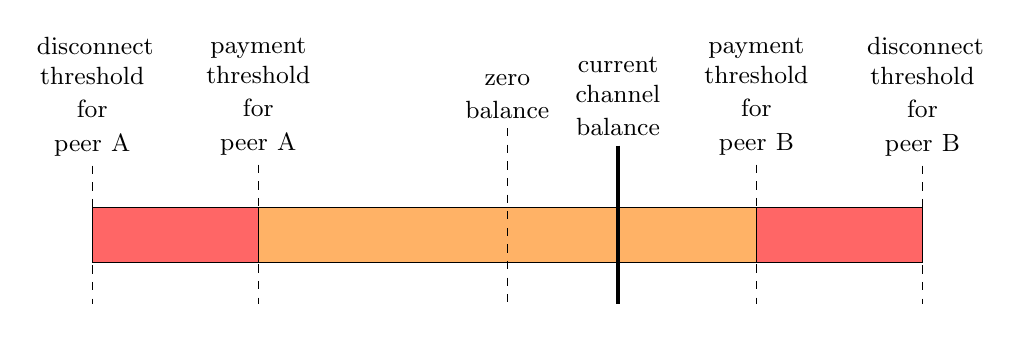
\begin{tikzpicture}
\node (middle)[draw, rectangle, fill=orange!60, minimum height=2em, minimum width=18em]{};
\node (leftred) [draw, rectangle, fill=red!60, minimum height=2em, minimum width=6em, node distance=12em,left of=middle]{};
\node (rightred)[draw, rectangle, fill=red!60, minimum height=2em, minimum width=6em, node distance=12em,right of=middle]{};
\node (zero) [above of=middle,node distance=5em, text width=4em, align=center] {\small zero\\ balance};
\node (zerod) [below of=middle] {};
\draw [dashed](zero)--(zerod);
\node (rtol) [node distance=9em,right of=zero,text width=4em, align=center] {\small payment\\threshold\\for peer B};
\node (rtold) [node distance=9em,right of=zerod] {};
\node (ltol) [node distance=9em,left of=zero,text width=4em, align=center] {\small payment\\threshold\\for peer A};
\node (ltold) [node distance=9em,left of=zerod] {};
\node (rdis) [node distance=15em, right of=zero,text width=4em, align=center] {\small disconnect\\threshold\\for peer B};
\node (rdisd) [node distance=15em,right of=zerod] {};
\node (ldis) [node distance=15em, left of=zero,text width=4em, align=center] {\small disconnect\\threshold\\for peer A};
\node (ldisd) [node distance=15em,left of=zerod] {};
\node (rbal) [node distance=4em,right of=zero,text width=4em, align=center] {\small current\\channel\\balance};
\node (rbald) [node distance=4em,right of=zerod] {};

\draw [dashed](rtol)--(rtold);
\draw [dashed](ltol)--(ltold);
\draw [dashed](rdis)--(rdisd);
\draw [dashed](ldis)--(ldisd);
\draw [very thick](rbal)--(rbald);
\end{tikzpicture}
\end{center}
\caption{Swap balance and swap thresholds.
Zero balance in the middle indicates consumption and provision are equal.
The current channel balance represents the difference in uncompensated service provision:
if to the right of zero, the balance tilts in favour of A with peer B being in debt, whereas to the left
the balance tilts in favour of B with A being in debt.
The orange interval represents loss tolerance. If the balance goes over the payment threshold, the party in
debt sends a cheque to its peer, if it reaches the disconnect threshold, the peer in debt is disconnected.}
\label{fig:swap}
\end{figure}
\end{center}

\subsubsection{Settling with payments}

In the presence of high variance, or unequal consumption of services, the balance will eventually tilt significantly toward one peer. In this situation, the indebted party issues a payment to the creditor to return the nominal balance to zero. This process is automatic and justifies swap as \emph{settle (the balance) with automated payments} (see figure \ref{fig:swap}). These payments can be just a commitments.

To quantify what counts as 'significant tilt', the swap protocol requires peers to advertise a \emph{payment threshold} $p$ as part of the handshake (\ref{spec:protocol:swap}): when their relative debt to their peer goes  above this threshold, they accept to be disconnected or not at least not served. So the reasonable  strategy is to pay earlier, already at $\frac{p}{n}$ (with $n=2$, called \emph{effective settlement threshold},  see \ref{spec:strategy:swap}). Sending the cheque and updating the  balance on the receiving side cannot be made an atomic operation without substantial added complexity. For instance, a client can  crash between receiving and processing the message, so even if the sending returns with no error, the sending peer can be sure the payment was received, this can result in discrepancies in accounting on the two sides. The tolerance of $\frac{(n-1)p}{n}$ is guarding against this, i.e., if the incidence of such crashes is not high and happen with roughly equal probability, the resulting minor discrepancies are shielded and not sanctioned.

\begin{center}
\begin{figure}[htbp]

\begin{center}
\begin{tabular}{ccc}
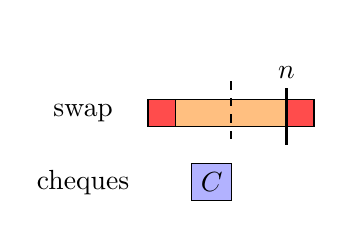
\begin{tikzpicture}
\node (middle)[draw, rectangle, fill=orange!50, minimum height=1em, minimum width=4em]{};
\node (leftred) [draw, rectangle, fill=red!70, minimum height=1em, minimum width=1em, node distance=2.5em, left of=middle]{};
\node (rightred)[draw, rectangle, fill=red!70, minimum height=1em, minimum width=1em, node distance=2.5em, right of=middle]{};
\node (zero) [above of=middle,node distance=2em, text height=1em] {};
\node (zerod) [below of=zero, node distance=3.5em] {};
\node (balance) [right of=zero,node distance=2em, text height=1.5em] {$n$};
\node (balanced) [below of=balance,node distance=3.5em] {};
\draw [dashed](zero)--(zerod);
\draw [very thick](balance)--(balanced);
\node (payment) [below of=zerod, node distance=1em]{};
\node (cheqeue) [draw, left of=payment, node distance=.7em, minimum height=1em, minimum width=1.4em, fill=blue!30, rectangle]{$C$};

\node (swap) [left of=leftred,minimum width=1em,align=right]{swap};
\node (cheques) [below of=swap,minimum width=1em, node distance= 2.5em, align=right]{cheques};
\end{tikzpicture}
&
\begin{tabular}{c}
  $\Longrightarrow$
\\ \\ \\ \\
\end{tabular}
&
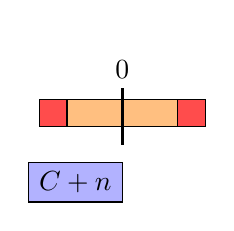
\begin{tikzpicture}
\node (middle)[draw, rectangle, fill=orange!50, minimum height=1em, minimum width=4em]{};
\node (leftred) [draw, rectangle, fill=red!70, minimum height=1em, minimum width=1em, node distance=2.5em, left of=middle]{};
\node (rightred)[draw, rectangle, fill=red!70, minimum height=1em, minimum width=1em, node distance=2.5em, right of=middle]{};
\node (zero) [above of=middle,node distance=2em, text height=1.5em] {$0$};
\node (zerod) [below of=zero, node distance=3.5em] {};
% \draw [dashed](zero)--(zerod);
\draw [very thick](zero)--(zerod);
\node (payment) [below of=zerod, node distance=1em]{};
\node (cheque) [draw, left of=payment, node distance=1.7em, minimum height=1em, minimum width=3.4em, fill=blue!30, rectangle]{$C+n$};
\end{tikzpicture}
\end{tabular}
\end{center}

\caption{Peer B's swap balance (with respect to A) reaches the payment threshold $n$ (left),
B sends a cheque to peer A. B keeps the cheque and restores the swap balance to zero.}
\label{fig:chequeswap}
\end{figure}
\end{center}

\subsection{Cheques}\label{sec:cheques}

One of the major issues with direct ``on-chain'' payments in a blockchain network is that each transaction must be processed by each and every node participating in the network, resulting in high transaction costs. One strategy to mitigate transaction costs is to defer payments and process them in bulk. In exchange for reduced cost, the beneficiary must be willing to incur higher risk of settlement failure. We argue that this is perfectly acceptable for bandwidth incentivisation where peers engage in repeated dealings.


\subsubsection{The chequebook contract}

A very simple smart contract that allows the beneficiary to choose when payments are to be processed was introduced in \cite{ethersphere2016sw3}. This \gloss{chequebook} contract is a wallet that can process cheques issued by its owner. The cheques are analogous to those in the real-world: the issuer signs a cheque specifying a beneficiary, a date and an amount, gives it to the recipient as a token of promise to pay at a later date. The smart contract plays the role of the bank. When the recipient wishes to get paid, they ``cash the cheque'' by submitting it to the smart contract. The contract, after validating the signature, date and the amount specified on the cheque, transfers the amount to the beneficiary's account (see figure \ref{fig:swap-chequebook}). Analogously to the person taking the cheque to the bank to cash it, anyone can send the digital cheque in a transaction to the owner's chequebook account and thus trigger the transfer. 

The swap protocol specifies that the payment sent when the \emph{effective settlement threshold} is exceeded, a cheque is sent over the creditor peer. Such cheques can be cashed immediately by being sent to the issuer's chequebook contract. Alternatively, cheques can also be withheld. Withholding a cheque is effectively lending on credit, which enables the parties to save on transaction costs. While, strictly speaking, there are no guarantees for solvency, nor is there an explicit punitive measure on insolvency, a bounced cheque will affect the issuer's reputation as the chequebook contract records it. On the premise that cheques are swapped in the context of repeating dealings, peers will refrain from issuing cheques beyond their balance. In other words, interest in keeping good reputation with their peers serves as an incentive for nodes to maintain solvency.


\begin{figure}[htbp]
\centering
% Agents
\def\IssuerLocal{A client}
\def\IssuerSwapContract{A swap}
\def\BeneficiarySwapContract{B swap}
\def\BeneficiaryLocal{B client}

% Message Flows
\def\Issue{issue cheque}% \def\Cheque{Cheque}
\def\Redeem{redeem cheque} %\def\Cheque{Cheque}
\def\Clear{clear ETH} %\def\ETH{ETH}
\def\NW{withdrawal event} %\def\Msg{Log Event}
\def\ND{deposit event} %\def\Msg{Log Event}

% Legend 
\def\LegendOnChain{On-chain}
\def\LegendOffChain{Off-chain}


\begin{tikzpicture}[every node/.style={font=\small,
  minimum height=.35cm,minimum width=.5cm},]

%
% Matrix
\node [matrix, very thin,column sep=1.0cm,row sep=0.2cm] (matrix) at (0,0) {
  & \node(0,0) (\IssuerLocal) {};   &                         & \node(0,0) (\IssuerSwapContract) {};   & & \node(0,0) (\BeneficiarySwapContract) {};   & & \node(0,0) (\BeneficiaryLocal) {}; \\
  & & & & & & & \\
  & & & & & & & \\
  & & & & & & & \\
  & \node(0,0) (\IssuerLocal 1) {}; & \node(0,0) (\Issue) {}; & \node(0,0) (\IssuerSwapContract 1) {}; & & \node(0,0) (\BeneficiarySwapContract 1) {}; & & \node(0,0) (\BeneficiaryLocal 1) {}; \\
  & & & & & & & \\
  & & & & & & & \\
  & \node(0,0) (\IssuerLocal 2) {}; &                         & \node(0,0) (\IssuerSwapContract 2) {}; & & \node(0,0) (\BeneficiarySwapContract 2) {}; & \node(0,0) (\Redeem) {};  &  \node(0,0) (\BeneficiaryLocal 2) {}; \\ 
  & & & & & & & \\
  & & & & & & & \\
  & \node(0,0) (\IssuerLocal 3) {}; &                         & \node(0,0) (\IssuerSwapContract 3) {}; & \node(0,0) (\Clear) {}; & \node(0,0) (\BeneficiarySwapContract 3) {}; &                    ; & \node(0,0) (\BeneficiaryLocal 3) {}; \\
  & & & & & & & \\
  & \node(0,0) (\IssuerLocal 4) {}; & \node(0,0) (\NW) {}   ; & \node(0,0) (\IssuerSwapContract 4) {}; &                         & \node(0,0) (\BeneficiarySwapContract 4) {}; & \node(0,0) (\ND) {}; & \node(0,0) (\BeneficiaryLocal 4) {}; \\
  & & & & & & & \\
  & \node(0,0) (\IssuerLocal 5) {}; &                         & \node(0,0) (\IssuerSwapContract 5) {};  & & \node(0,0) (\BeneficiarySwapContract 5) {};& & \node(0,0) (\BeneficiaryLocal 5) {}; \\
  & & & & & & & \\
  & \node(0,0) (\IssuerLocal 6) {}; &                         & \node(0,0) (\IssuerSwapContract 6) {};  & & \node(0,0) (\BeneficiarySwapContract 6) {};& & \node(0,0) (\BeneficiaryLocal 6) {}; \\
  & & & & & & & \\
  & \node(0,0) (\IssuerLocal 7) {}; & \node(0,0) (\LegendOnChain) {};  & & & & & \\
  & \node(0,0) (\IssuerLocal 8) {}; & \node(0,0) (\LegendOffChain) {}; & & & & & \\
};

% Agents labels
\fill 
	(\IssuerLocal) node[draw,fill=white] {\IssuerLocal}
	(\IssuerSwapContract) node[draw,fill=white] {\IssuerSwapContract}
	(\BeneficiarySwapContract) node[draw,fill=white] {\BeneficiarySwapContract}
	(\BeneficiaryLocal) node[draw,fill=white] {\BeneficiaryLocal};

\draw [dashed] 
  (\IssuerLocal) -- (\IssuerLocal 6)
  (\BeneficiaryLocal) -- (\BeneficiaryLocal 6)
  (\IssuerSwapContract) -- (\IssuerSwapContract 6)
  (\BeneficiarySwapContract) -- (\BeneficiarySwapContract 6);

% Horizontal flows (Monetary interactions)
%\draw [-latex] (\IssuerLocal 1) -- (\IssuerSwapContract 1.west) arc(180:0:0.37cm) -- (\BeneficiarySwapContract 1.west) arc(180:0:0.37cm) -- (\BeneficiaryLocal 1);
\draw [-{Latex[length=1.5mm,width=2.5mm]}] (\IssuerLocal 1) -- (\BeneficiaryLocal 1);
\draw [-{Latex[length=1.5mm,width=2.5mm]}] (\BeneficiaryLocal 2) -- (\IssuerSwapContract 2);
%\draw [-latex] (\BeneficiaryLocal 2) -- (\BeneficiarySwapContract 2.east) arc(0:180:0.37cm) -- (\IssuerSwapContract 2);
\draw [-{Latex[length=1.5mm,width=2.5mm]}] (\IssuerSwapContract 3) -- (\BeneficiarySwapContract 3);
\draw [-{Latex[length=1.5mm,width=2.5mm]}] (\IssuerSwapContract 3) -- (\IssuerLocal 4);
\draw [-{Latex[length=1.5mm,width=2.5mm]}] (\BeneficiarySwapContract 3) -- (\BeneficiaryLocal 5);

% Flows Labels 
\fill
  (\Issue) 
    node[above, font=\footnotesize ] {\Issue}
  (\Redeem) 
    node[above, font=\footnotesize] {\Redeem}
  (\Clear) 
    node[above, font=\footnotesize] {\Clear}
  (\NW) 
    node[above, font=\footnotesize, text width=1.4cm, text height=1.5cm, align=center,fill=white] {\NW}
  (\ND) 
    node[above, font=\footnotesize, text width=1.5cm,align=center,fill=white] {\ND};

% Interaction points 
\draw 
  (\IssuerLocal 1) node[minimum size=0.25cm, draw,circle,fill=red!20] {}
  (\BeneficiaryLocal 1) node[minimum size=0.25cm, draw,circle,fill=red!20] {}
  (\BeneficiaryLocal 2) node[minimum size=0.25cm, draw,circle,fill=red!20] {}
  (\IssuerSwapContract 2) node[minimum size=0.25cm, draw,circle,fill=green!20] {}
  (\IssuerSwapContract 3) node[minimum size=0.25cm, draw,circle,fill=green!20] {}
  (\IssuerLocal 4) node[minimum size=0.25cm, draw,circle,fill=red!20] {}
  (\BeneficiarySwapContract 3) node[minimum size=0.25cm, draw,circle,fill=green!20] {}
  (\BeneficiaryLocal 5) node[minimum size=0.25cm, draw,circle,fill=red!20] {}
  (\IssuerLocal 7) node[minimum height=.1cm, minimum size=0.1cm, draw,circle,fill=green!20] {}
  (\IssuerLocal 8) node[minimum height=.1cm, minimum size=0.1cm, draw,circle,fill=red!20] {};

% Vertical lifelines
\draw [-{Latex[length=1.5mm,width=2mm]}] (\IssuerSwapContract 2) -- (\IssuerSwapContract 3);
 Legend labels
\draw
	(\LegendOnChain) node[minimum height=.1cm] {\LegendOnChain}
	(\LegendOffChain) node[minimum height=.1cm] {\LegendOffChain};
\end{tikzpicture}

\caption{The basic interaction sequence for swap chequebooks}
\label{fig:swap-chequebook}
\end{figure}


\subsubsection{Double cashing}

Since these digital cheques are files and can therefore be copied, care must be taken that the same cheque cannot be cashed twice. Such ``double cashing'' can be prevented by assigning each cheque given to a particular beneficiary a serial number which the contract will store when the cheque is cashed. The chequebook contract can then rely on the serial number to make sure cheques are cashed in sequential order, thus needing to store only a single serial number per beneficiary.

An alternative strategy to prevent double cashing, when repeated payments are made to the same beneficiary, is that the cheques contain the \emph{cumulative} total amount ever credited to the beneficiary. The total cumulative amount that has been cashed out is stored in the contract for each beneficiary. When a new cheque is submitted, the contract ignores cheques with amount equal to or less than the stored total, but it will transfer the difference if it receives a cheque with a higher total.


This simple trick also makes it possible to cash cheques in bulk because only the current `last cheque' need ever be processed. This achieves the reduction of transaction costs alluded to above.

The amount deposited in the chequebook (\gloss{global balance}) serves as collateral for the cheques. It is pooled over the beneficiaries of all outstanding cheques. In this simplest form, the chequebook has the same guarantee as real-world cheques: none. Since funds can be freely moved out of the chequebook wallet at any time, solvency at the time of cashing can never be guaranteed: if the chequebook's balance is less than the amount sanctioned by a cheque submitted to it, the cheque will bounce. This is the trade off between transaction costs and risk of settlement failure.

\subsection{Waivers}\label{sec:waiver}

If the imbalance in the swap channel is the result of high variance as opposed to unequal consumption, after a period of accumulating cheques the channel balance starts tilting the other way. Normally it is now up to the other party to issue cheques to its peer resulting in uncashed cheques accumulating on both sides.
To allow for further savings in transaction costs, it could be desirable to be able to `play the cheques off against each other'.

Such a process is possible, but it requires certain important changes within the chequebook contract. In particular, cashing cheques can no longer be immediate and must incur a security delay, familiar from payment channels.

Let us imagine a system analogous to cheques being returned to the issuer. Assume peer A issued cheques to B and the balance was brought back to zero. Later the balance tilts in A's favour but the cheques from A to B have not been cashed. In the real world, user B could simply return the last cheque back to A or provably destroy it. In our case it is not so simple; we need some other mechanism by which B  \emph{commits not to cash} that particular cheque. Such a commitment could take several forms; it could be implemented by B signing a message allowing A to issue a new `last cheque` which has a lower cumulative total amount than before, or perhaps B can issue some kind of `negative` cheque for A's chequebook that would have the effect as if a cheque with the same amount had been paid. 

What all the implementations have in common, is that the chequebook can no longer allow instantaneous cashing of cheques. Upon receiving a cheque cashing request, the contract must wait to allow the other party in question to submit potentially missing information about cancelled cheques or reduced totals. To accommodate (semi-)bidirectional payments using a single chequebook we make the following modifications:

\begin{enumerate}
    \item All cheques from user A to user B must contain a serial number.
    \item Each new cheque issued by A to B must increase the serial number.
    \item A's chequebook contract records the serial number of the last cheque that B cashed.
    \item During the cashing delay, valid cheques with higher serial number supersede any previously submitted cheques regardless of their face value.
    \item Any submitted cheque which decreases the payout of the previously submitted cheque is only valid if it is signed by the beneficiary.
\end{enumerate}


\begin{figure}[htbp]
\centering
% Waivers diagram 
% Author: Fabio Barone, based on Pascal Seppecher taken from http://www.texample.net/tikz/examples/sequence-diagram/

% Agents
\def\A{A}
\def\B{B}
\def\FaceVal{Amount due}
\def\Contract{Contract value}
\def\Totals{Cumulative Sum}

% Message Flows
\def\ChequeA{Cheque $c0$}
\def\ChequeB{Cheque $c1$}
\def\ChequeC{Cheque $c2$}
\def\RedeemC{Redeem Cheque $c1$}
\def\ChequeD{Cheque $c3$}
\def\WFailCumTotTooHigh{Waive attempt $w_4$}
\def\WaiverA{Waive $w_4$}
\def\RedeemFailWrongSN{Redeem $c3$}
\def\WaiverB{Waive $w_5$}
\def\ChequeE{Cheque $c6$}
\def\ChequeF{Cheque $c7$}
\def\RedeemF{Redeem $c7$}
\def\ChequeG{Cheque $c8$}
\def\RedeemG{Redeem $c8$}

% Legend 
%\def\LegendOnChain{On-chain}
%\def\LegendOffChain{Off-chain}

\begin{tikzpicture}[every node/.style={font=\small,
  minimum height=.35cm,minimum width=.5cm}]
 \useasboundingbox (-1cm,-7cm) rectangle (3.5cm,7cm);
   \scope[transform canvas={scale=.75}]


%
% Matrix
\node [matrix, very thin,column sep=2.0cm,row sep=0.4cm] (matrix) at (0,0) {
  &  & \node(0,0) (\A) {}; &                        & \node(0,0) (\B) {};        & \node(0,0) {Serial};               & \node(0,0) (\FaceVal) {};  & \node(0,0) (\Contract) {}; & \node(0,0) (\Totals) {}; \\
  &  & & & & & & &  \\
  &  & & & & & & &  \\
  &  & & & & & & & \\
  &  & \node(0,0) (\A 1) {}; & \node(0,0) (\ChequeA) {}; & \node(0,0) (\B 1) {};& \node(0,0) {0};                    & \node(0,0) {6};          & \node(0,0) {6};            & \node(0,0) {6}; \\
  &  & & & & & & & \\
  &  & \node(0,0) (\A 2) {}; & \node(0,0) (\ChequeB) {}; & \node(0,0) (\B 2) {};& \node(0,0) {1};                     & \node(0,0) {9};          & \node(0,0) {15};            & \node(0,0) {15}; \\ 
  &  & & & & & & & \\
  &  & \node(0,0) (\A 3) {}; & \node(0,0) (\ChequeC) {}; & \node(0,0) (\B 3) {};& \node(0,0) {2};                     & \node(0,0) {13};          & \node(0,0) {28};            & \node(0,0) {28}; \\
  &  & & & & & & & \\
  &  & \node(0,0) (\A 4) {}; & \node(0,0) (\RedeemC) {}; & \node(0,0) (\B 4) {};& \node(0,0) {1};                 & \node(0,0) {15};          & \node(0,0) {19};            & \node(0,0) {28}; \\
  &  & & & & & & & \\
  &  & \node(0,0) (\A 5) {}; & \node(0,0) (\ChequeD) {}; & \node(0,0) (\B 5) {};& \node(0,0) {3};                     & \node(0,0) {14};          & \node(0,0) {33};            & \node(0,0) {42}; \\
  & & & & & & & & \\
  & \node(0,0) {Fails as exceeds Contract value} ;  & \node(0,0) (\A 6) {}; & \node(0,0) (\WFailCumTotTooHigh) {}; & \node(0,0) (\B 6) {}; & \node(0,0) {4};    & \node(0,0) {100};          & \node(0,0) {33};            & \node(0,0) {42}; \\
  &  & & & & & & & \\
  &  & \node(0,0) (\A 7) {}; & \node(0,0) (\WaiverA) {}; & \node(0,0) (\B 7) {};& \node(0,0) {4};                     & \node(0,0) {7};          & \node(0,0) {26};            & \node(0,0) {42}; \\
  &  & & & & & & & \\
  & \node(0,0) {Fails due to wrong s/n}; & \node(0,0) (\A 8) {}; & \node(0,0) (\RedeemFailWrongSN) {}; & \node(0,0) (\B 8) {};& \node(0,0) {3};      & \node(0,0) {42};          & \node(0,0) {26};            & \node(0,0) {42}; \\
  &  & & & & & & & \\
  &  & \node(0,0) (\A 9) {}; & \node(0,0) (\WaiverB) {}; & \node(0,0) (\B 9) {};& \node(0,0) {5};                     & \node(0,0) {26};          & \node(0,0) {0};            & \node(0,0) {42}; \\
  &  & & & & & & & \\
  &  & \node(0,0) (\A 10) {}; & \node(0,0) (\ChequeE) {}; & \node(0,0) (\B 10) {};& \node(0,0) {6};                     & \node(0,0) {11};          & \node(0,0) {11};            & \node(0,0) {53}; \\
  &  & & & & & & & \\
  &  & \node(0,0) (\A 11) {}; & \node(0,0) (\ChequeF) {}; & \node(0,0) (\B 11) {};& \node(0,0) {7};                     & \node(0,0) {15};          & \node(0,0) {26};            & \node(0,0) {68}; \\
  &  & & & & & & & \\
  &  & \node(0,0) (\A 12) {}; & \node(0,0) (\RedeemF) {}; & \node(0,0) (\B 12) {};& \node(0,0) {7};               & \node(0,0) {68};          & \node(0,0) {0};            & \node(0,0) {68}; \\
  &  & & & & & & & \\
  & \node(0,0) {Exchange in other direction ok};   & \node(0,0) (\A 13) {}; & \node(0,0) (\ChequeG) {}; & \node(0,0) (\B 13) {};& \node(0,0) {0};                     & \node(0,0) {};          & \node(0,0) {};            & \node(0,0) {}; \\
  &  & & & & & & & \\
  &  & \node(0,0) (\A 14) {}; & \node(0,0) (\RedeemG) {}; & \node(0,0) (\B 14) {}; & \node(0,0) {1};              & \node(0,0) {};          & \node(0,0) {};            & \node(0,0) {}; \\
  &  & & & & & & & \\
  &  & \node(0,0) (\A 15) {}; &                          ; & \node(0,0) (\B 15) {};&                               &                           &                             &                  \\
};

% Agents labels
\fill 
	(\A) node[draw,fill=white] {\A}
	(\B) node[draw,fill=white] {\B}
	(\FaceVal) node[] {\FaceVal}
	(\Contract) node[] {\Contract}
	(\Totals) node[] {\Totals};

\draw [dashed] 
  (\A) -- (\A 15)
  (\B) -- (\B 15);

% Horizontal flows 
\draw [-{Latex[length=1.5mm,width=2.5mm]}] (\A 1) -- (\B 1);
\draw [-{Latex[length=1.5mm,width=2.5mm]}] (\A 2) -- (\B 2);
\draw [-{Latex[length=1.5mm,width=2.5mm]}] (\A 3) -- (\B 3);
\draw [-{Latex[length=1.5mm,width=2.5mm]}] (\B 4) -- (\A 4);
\draw [-{Latex[length=1.5mm,width=2.5mm]}] (\A 5) -- (\B 5);
\draw [-{Latex[length=1.5mm,width=2.5mm]},color=red] (\B 6) -- (\A 6);
\draw [-{Latex[length=1.5mm,width=2.5mm]}] (\B 7) -- (\A 7);
\draw [-{Latex[length=1.5mm,width=2.5mm]},color=red] (\B 8) -- (\A 8);
\draw [-{Latex[length=1.5mm,width=2.5mm]}] (\B 9) -- (\A 9);
\draw [-{Latex[length=1.5mm,width=2.5mm]}] (\A 10) -- (\B 10);
\draw [-{Latex[length=1.5mm,width=2.5mm]}] (\A 11) -- (\B 11);
\draw [-{Latex[length=1.5mm,width=2.5mm]}] (\B 12) -- (\A 12);
\draw [-{Latex[length=1.5mm,width=2.5mm]}] (\A 13) -- (\B 13);
\draw [-{Latex[length=1.5mm,width=2.5mm]}] (\B 14) -- (\A 14);

% Flows Labels 
\fill
  (\ChequeA) 
    node[above] {\ChequeA}
  (\ChequeB) 
    node[above] {\ChequeB}
  (\ChequeC) 
    node[above] {\ChequeC}
  (\RedeemC) 
    node[above] {\RedeemC}
  (\ChequeD) 
    node[above] {\ChequeD}
  (\WFailCumTotTooHigh) 
    node[above] {\WFailCumTotTooHigh}
  (\WaiverA) 
    node[above] {\WaiverA}
  (\RedeemFailWrongSN) 
    node[above] {\RedeemFailWrongSN}
  (\WaiverB) 
    node[above] {\WaiverB}
  (\ChequeE) 
    node[above] {\ChequeE}
  (\ChequeF) 
    node[above] {\ChequeF}
  (\RedeemF) 
    node[above] {\RedeemF}
  (\ChequeG) 
    node[above] {\ChequeG}
  (\RedeemG) 
    node[above] {\RedeemG};

% Interaction points 
\draw 
  (\A 1) node[minimum size=0.25cm, draw,circle,fill=red!20] {}
  (\B 1) node[minimum size=0.25cm, draw,circle,fill=red!20] {}
  (\A 2) node[minimum size=0.25cm, draw,circle,fill=red!20] {}
  (\B 2) node[minimum size=0.25cm, draw,circle,fill=red!20] {}
  (\A 3) node[minimum size=0.25cm, draw,circle,fill=red!20] {}
  (\B 3) node[minimum size=0.25cm, draw,circle,fill=red!20] {}
  (\A 4) node[minimum size=0.25cm, draw,circle,fill=red!20] {}
  (\B 4) node[minimum size=0.25cm, draw,circle,fill=red!20] {}
  (\A 5) node[minimum size=0.25cm, draw,circle,fill=red!20] {}
  (\B 5) node[minimum size=0.25cm, draw,circle,fill=red!20] {}
  (\A 6) node[minimum size=0.25cm, draw,circle,fill=red!20] {}
  (\B 6) node[minimum size=0.25cm, draw,circle,fill=red!20] {}
  (\A 7) node[minimum size=0.25cm, draw,circle,fill=red!20] {}
  (\B 7) node[minimum size=0.25cm, draw,circle,fill=red!20] {}
  (\A 8) node[minimum size=0.25cm, draw,circle,fill=red!20] {}
  (\B 8) node[minimum size=0.25cm, draw,circle,fill=red!20] {}
  (\A 9) node[minimum size=0.25cm, draw,circle,fill=red!20] {}
  (\B 9) node[minimum size=0.25cm, draw,circle,fill=red!20] {}
  (\A 10) node[minimum size=0.25cm, draw,circle,fill=red!20] {}
  (\B 10) node[minimum size=0.25cm, draw,circle,fill=red!20] {}
  (\A 11) node[minimum size=0.25cm, draw,circle,fill=red!20] {}
  (\B 11) node[minimum size=0.25cm, draw,circle,fill=red!20] {}
  (\A 12) node[minimum size=0.25cm, draw,circle,fill=red!20] {}
  (\B 12) node[minimum size=0.25cm, draw,circle,fill=red!20] {}
  (\A 13) node[minimum size=0.25cm, draw,circle,fill=red!20] {}
  (\B 13) node[minimum size=0.25cm, draw,circle,fill=red!20] {}
  (\A 14) node[minimum size=0.25cm, draw,circle,fill=red!20] {}
  (\B 14) node[minimum size=0.25cm, draw,circle,fill=red!20] {};

% Vertical lifelines
\endscope
\end{tikzpicture}

\caption{Example sequence of mixed cheques and waivers exchange}
\label{fig:waivers-diagram}
\end{figure}

With these rules in place it is easy to see how cheque cancellation would work. Suppose user A has issued cheques $c_0 \ldots c_n$ with cumulative totals $t_0 \ldots t_n$ to user B. Suppose that the last cheque B cashed was $c_i$. The chequebook contract has recorded that B has received a payout of $t_i$ and that the last cheque cashed had serial number $i$.

Let us further suppose that the balance starts tilting in A's favour by some amount $x$. If B had already cashed cheque $c_n$, then B would now have to issue a cheque of her own using B's chequebook as the source and naming A as the beneficiary. However, since cheques $c_{i+1} \ldots c_n$  are uncashed, B can instead send to A a cheque with A's chequebook as the source, B as the beneficiary, with serial number $n+1$ and cumulative total $t_{n+1} = t_n - x$. Due to the rules enumerated above, A will accept this as equivalent to a payment of amount $x$ by B.  In this scenario, instead of sending a cheque to A, B waive part of their earlier entitlement. This justifies swap as \emph{send waiver as payment}.

This process can be repeated multiple times until the cumulative total is brought back to $t_i$. At this point all outstanding debt has effectively been cancelled and any further payments must be made in the form of a proper cheque from B's chequebook to A (See figure \ref{fig:waivers-diagram}).


\subsection{Zero capital entry}\label{sec:zero-capital-entry}

Swap accounting can also work in one direction only. If a party enters the system with zero liquid capital (\gloss{newcomer}), but connects to peers with funds (\gloss{insider}), the newcomer begins to provide the service (and not use it) in order to earn a positive swap balance. Once the payment threshold is reached, the newcomer will be paid and is soon able to deploy chequebook of her own.
In short, even without any chequebook contract at all, Swap offers zero-capital onboarding to newcomers. Once the payout threshold is reached, the insiders could pay the newcomers on-chain. 

If the insider has a chequebook and wishes to pay the newcomer with a cheque, this is also possible, but there is a caveat here in that cashing cheques requires sending a transaction to the blockchain, and therefore: gas.%
%
\footnote{Although this restriction may be dropped once ethereum is upgraded to allow the chequebook contract will be able to pay for the transfer and deduct the cost of the transfer from the payout.}
%
The newcomer will be able to earn cheques for services provided, but will not have the means to cash them. 
Unless the first payment is an on-chain payment or the node can convince one of its peers to send the transaction for them.

We allow nodes to sign off on a structure that they want spent, and extend the swap contract with a preprocessing step, which triggers payment to the transaction sender covering the transaction's gas cost plus a service fee. 



\begin{figure}[htbp]
\centering
% Chequebook diagram 
% Author: Fabio Barone, based on Pascal Seppecher taken from http://www.texample.net/tikz/examples/sequence-diagram/


% Agents
\def\Legend{}
\def\Newcomer{Newcomer}
\def\NewcomerSwap{Newcomer swap}
\def\Insider{Insider}
\def\InsiderSwap{}

% Message Flows
\def\Connect{Connect}
\def\Consume{Consume service}
\def\CreateContract{Create contract} 

% Legend 
\def\ContractCreationThreshold{Contract creation threshold reached} 
   
\begin{tikzpicture}[every node/.style={font=\small,
  minimum height=.35cm,minimum width=.5cm},]

%
% Matrix
\node [matrix, very thin,column sep=1.2cm,row sep=0.8cm] (matrix) at (0,0) {
  & \node(0,0) (\Legend)[column sep=2cm] {};   & \node(0,0) (\Newcomer) {};   &                           & \node(0,0) (\NewcomerSwap) {};   &                          & \node(0,0) (\Insider) {}; & & \node(0,0) (\InsiderSwap) {}; \\
  & & & & & & & & \\
  & \node(0,0) (\Legend 1) {}; & \node(0,0) (\Newcomer 1) {}; & \node(0,0) (\Connect){};  & \node(0,0) (\NewcomerSwap 1) {}; &                          & \node(0,0) (\Insider 1) {}; & & \node(0,0) (\InsiderSwap 1) {}; \\
  & \node(0,0) (\Legend 2) {}; & \node(0,0) (\Newcomer 2) {}; &                           & \node(0,0) (\NewcomerSwap 2) {}; & \node(0,0) (\Consume){}; & \node(0,0) (\Insider 2) {}; & &  \node(0,0) (\InsiderSwap 2) {}; \\ 
  & \node(0,0) (\Legend 3) {}; & \node(0,0) (\Newcomer 3) {}; &                           & \node(0,0) (\NewcomerSwap 3) {}; & \node(0,0) (\Consume 1){}; & \node(0,0) (\Insider 3) {}; & &  \node(0,0) (\InsiderSwap 3) {}; \\ 
  & & & & & & & & \\
  & \node(0,0) (\ContractCreationThreshold) {}; & \node(0,0) (\Newcomer 4) {}; &          & \node(0,0) (\NewcomerSwap 4) {}; & \node(0,0) (\Consume 2){}; & \node(0,0) (\Insider 4) {}; & &  \node(0,0) (\InsiderSwap 4) {}; \\ 
  & \node(0,0) (\Legend 5) {}; & \node(0,0) (\Newcomer 5) {}; &                           & \node(0,0) (\NewcomerSwap 5) {}; & \node(0,0) (\CreateContract){};  & \node(0,0) (\Insider 5) {}; & &  \node(0,0) (\InsiderSwap 4) {}; \\ 
  & \node(0,0) (\Legend 6) {}; & \node(0,0) (\Newcomer 6) {}; &                           & \node(0,0) (\NewcomerSwap 6) {}; &                          & \node(0,0) (\Insider 6) {};& & \node(0,0) (\InsiderSwap 6) {}; \\
};

% Agents labels
\fill 
	(\Newcomer) node[draw,fill=white] {\Newcomer}
	(\NewcomerSwap) node[draw,fill=white] {\NewcomerSwap}
	(\Insider) node[draw,fill=white] {\Insider};

\draw [dashed] 
  (\NewcomerSwap) -- (\NewcomerSwap 6)
  (\Newcomer) -- (\Newcomer 6)
  (\Insider) -- (\Insider 6);

% Horizontal flows (Monetary interactions)
\draw [-{Latex[length=1.5mm,width=2.5mm]}] (\Newcomer 1) -- (\Insider 1);
\draw [-{Latex[length=1.5mm,width=2.5mm]}] (\Insider 2) -- (\Newcomer 2);
\draw [-{Latex[length=1.5mm,width=2.5mm]}] (\Insider 3) -- (\Newcomer 3);
\draw [-{Latex[length=1.5mm,width=2.5mm]}] (\Insider 4) -- (\Newcomer 4);
\draw [-{Latex[length=1.5mm,width=2.5mm]}] (\Insider 5) -- (\NewcomerSwap 5);

% Flows Labels 
\fill
  (\Connect) 
    node[above] {\Connect}
  (\Consume) 
    node[above] {\Consume}
  (\Consume 1) 
    node[above] {\Consume}
  (\Consume 2) 
    node[above] {\Consume}
  (\CreateContract) 
    node[above] {\CreateContract}
  (\ContractCreationThreshold) 
    node[text width=1.5cm] {\ContractCreationThreshold};

% Interaction points 
\draw 
  (\Newcomer 1) node[minimum size=0.25cm, draw,circle,fill=red!20] {}
  (\Insider 1) node[minimum size=0.25cm, draw,circle,fill=red!20] {}
  (\Newcomer 2) node[minimum size=0.25cm, draw,circle,fill=red!20] {}
  (\Insider 2) node[minimum size=0.25cm, draw,circle,fill=red!20] {}
  (\Newcomer 3) node[minimum size=0.25cm, draw,circle,fill=red!20] {}
  (\Insider 3) node[minimum size=0.25cm, draw,circle,fill=red!20] {}
  (\Newcomer 4) node[minimum size=0.25cm, draw,circle,fill=red!20] {}
  (\Insider 4) node[minimum size=0.25cm, draw,circle,fill=red!20] {}
  (\NewcomerSwap 5) node[minimum size=0.25cm, draw,circle,fill=red!20] {}
  (\Insider 5) node[minimum size=0.25cm, draw,circle,fill=red!20] {};

% Vertical lifelines

\end{tikzpicture}

\caption{Bootstrapping or how to launch as a swap capable node consuming and providing a
service and earn money}
\label{fig:zero-cost-entry}
\end{figure}

  
A newcomer connects to  an insider with an existing chequebook contract. The insider consumes the newcomer's services and instead of issuing a cheque, the insider agrees to create a chequebook contract for the newcomer. When the insider's service debt reaches the amount needed for contract creation, the insider sends a transaction to create the contract with newcomer as the owner. Once the newcomer has her own chequebook contract, she is able to consume services and issue cheques to pay for them.
 
In order to be useful, however, the deployed chequebook must also have some positive balance as collateral. Since the newcomer has no liquid capital, it must be the insiders who deposit this starting balance. If peers agreed that they want to save on transaction costs, it is reasonable to create the contract with the required initial balance in one go. This would imply waiting out with contract creation until the insider's debt reaches the \emph{cost of bootstrapping} which is the sum of (1) the cost of contract creation, (2) the required starting balance, and (3) possibly some extra service fee to incentivise insiders to provide this kind of service (see figure \ref{fig:zero-cost-entry}). This feature jusitfies swap as \emph{start without a penny, setup a wallet as payment}.

\section{Storage incentives}\label{sec:storage-incentives}

In \ref{sec:postage-stamps}, we introduce postage stamps, primarily as a measure against spam protection. In \ref{sec:capacity-pressure} describes how the pricing mechanism can be used to signal capacity pressure of the network and how the incentives work to rectify that. 
We then turn to postage lottery explaining how postage stamps used for spam protection can be modified to give positive incentives to nodes to store files and indicate their importance via price (\ref{sec:postage-lottery}). Finally \ref{sec:chunk-insurance} shows how positive rewards of the postage lottery can be complemented by introducing staked insurers who stand to lose their deposit if they lose chunks they insured. We argue that such punitive measures are crucial in mitigating the tragedy of commons problem in systems with positive storage incentives only. 

\subsection{Spam protection with postage stamps}\label{sec:postage-stamps}

Syncing involves transferring chunks from the uploader to storers, i.e., to the neighbourhood where the chunk falls within the nodes' area of responsibility. Storer nodes aspire to serve content as a response to retrieve requests. All else being equal, given kademlia routing, the closer a node is to the chunk address, the more likely it is that a request for that chunk will end up with them. This creates a weak incentive for storer nodes to sync content. However, it presupposes that the chunk has the promise of some profit. This assumption is broken if an adversary spams the network with chunks (maybe randomly generated) never requested by anyone. Attaching a cost to uploading a chunk to swarm can mitigate such an attack. 


\subsubsection{Postage stamps}

Taking inspiration from international mail delivery, the entire delivery path (as well as storage) can be pre-paid and the proof of payment called a \gloss{postage stamp} needs to be attached to the payload by the sender.

This cost need not necessarily be borne by the uploaders but they are the ones that need to make sure the postage stamp is attached to each chunk,  otherwise the upload willl not succeed. Conversely,  the inpayment need not necessarily be paid out as revenue to anyone in particular, i.e., it can be burnt or otherwise redistributed. The actual cost of uploading a chunk can serve as a signal of importance (somewhat analogously to priority mail) which storer nodes can also use to rank chunks when selecting which one to garbage collect (see \ref{spec:strategy:garbage-collection}) in the event of capacity shortage.



\subsubsection{Proof of payment}

The proof of payment can lend itself to a number of different implementations. The most obvious choice is to make payments to a central postage stamp issuer smart contract on the blockchain.%
%
\footnote{Using a cheque seems one option, however, cheques are  signed against cumulative debt and therefore assume the single beneficiary is able to reconstruct the added value over the previously sent cheque. In other words, cheques are not appropriate to communicate value to non-peers.}
%
Because of the high transaction cost, requiring an on-chain payment for each chunk is prohibitively expensive. Instead we need a solution that allows the uploader to purchase the postage stamp in a \emph{batch} and reuse it over several chunks. 

The postage stamp batch is associated with the following components:

\begin{itemize}
\item \emph{payment identifier} - a reference generated for  the batch when payment is made
\item \emph{owner address} - the owner that is entitled to sign the batch with a chunk address
\item \emph{balance} - total amount available for the batch
\item \emph{batch size} - the number of times the same payment/batch can be used for stamping chunks
\item \emph{payout rate} - unit price meant for a chunk per block 
\end{itemize}


When the payment is created, an owner address is set that is allowed to attach stamps to chunks. Also a \emph{payout rate} - unit price of a chunk per block is specified for the batch, the payout rate times batch size must not exceed the amount paid. If the payment is successful a payment id is assigned representing the paid batch. 

Anyone can top up a postage stamp at a later date and decide if part of the funds are spent on increasing the payout rate. Decreasing the payout rate is not possible. 

The postage stamp attached to a chunk is a data structure with the following fields (see more detail in \ref{spec:format:postage-stamps}):

\begin{itemize}
    \item \emph{chunk address} - the address the stamp is attached to 
    \item \emph{payment identifier} - a reference that can be checked with the smart contract
    \item \emph{witness} - signature linking the stamp and the address 
\end{itemize}

\subsubsection{Validity}

An actual postage stamp is valid for a chunk if it is (1) signed by the address specified for the payment identifier according to the smart contract, (2) the address of the chunk it is attached to matches the one on the stamp, and (3) it has not exhausted its balance.

\subsubsection{Value density of postage batches}

The \emph{value density} of a postage stamp is measured in honey/blocktime/chunk and is obtained by dividing the current balance of the batch by the batch size and the number of blocks passed since the last out payment. Similarly to stamps used for postal mail, a single chunk can have multiple postage stamps attached to it. In this case the value densities conferred to the chunk by valid postage stamps simply add up. 

\subsubsection{Validating batch size}

Note that the value density depends on the batch size which is self declared by the user, so without further measures, it allows for an overspend attack in which the uploader reuses the stamp over many more chunks than the self-acclaimed batch size and trick the unsuspect storers into underpaid extra work. The question arises  
how we can prevent a malicious uploader from signing more chunks with the same postage stamp than they claim in the batch size. In the absence of global visibility of all chunks signed with a postage stamp: nodes cannot directly verify the value density, as they have no access to postage stamps attached to chunks that do not pass through them. 

There needs to be a way for nodes to assess value densities based only locally available information, notably relying on chunks with the same postage stamp that they do have.%
%
\footnote{One solution is based on the realisation that estimation of absolute value densities is strictly speaking unnecessary. Nodes only want to prioritize chunks in case of resource shortage and for ranking chunks, comparison of the relative value densities of postage stamps that they have is sufficient.  This relative density is calculated by taking the number of chunks sharing the same postage stamp in the node's local storage. The reason this is a good enough strategy is apparent if we investigate how the uploader can manipulate the relative rank of their postage. If these cardinalities are uniform across nodes, then the estimation is both correct and consensual. Given chunk addresses are uniformly distributed, if chunks are randomly assigned to available postage stamps, on average an equal number of chunks will land in every neighbourhood. All the malicious uploader can do is artificially increase the density in certain neighbourhoods. However, such  manipulation can only lead to a situation where the target neighbourhood underestimates the relative value of the postage stamps. This will result in a lower rank for the chunks using the same stamp leading to earlier garbage collection and can ultimately only  hurt  the uploader.}

\subsubsection{Limiting batch size by constraining prefix collisions}

The solution is to impose an explicit uniformity requirement on the batches. We define the \emph{depth} of a postage batch as the logarithm of its size, and we posit the constraint that chunks signed with the same batch identifier have no \emph{prefix collision} longer than the depth. A postage stamp with a batch size of $2^d$ can be thought of as a balanced binary tree of depth $d$, where the leaves correspond to maximum length \emph{collision slots} of the batch. If the depth of a batch is greater than the depth of the network (the number of nodes $N<2^n$), then all chunks matching the same collision slot are guaranteed to land in the same neighbourhoods, and, as a result, "violations" of the uniformity requirement will be locally detected by nodes. If they respond to this violation by randomly keeping only one of the chunks for each collision slot, uploaders will not only lose one chunk but also some predictability on top.

Since chunk addresses will have a variance, in practice an uploader will need to use a set of postage batches and when it needs to attach a postage stamp to a chunk, it finds one with an unfilled collision slot for the chunk address in question.  In general, the best utilisation of the stamp is filling all the different collision slots (see \ref{sec:upload}). Put differently, continued non-uniformity will lead to underutilised stamps and therefore higher unit price for uploading and storing a chunk. This solution has the desired side effect that it imposes an upfront cost to non-uniform uploads: the more focussed our upload is on a neighbourhood, the more slots of the postage stamps remain unused. As a consequence, directing uploads to a neighbourhood is expensive.%
%
\footnote{The cost of targeted attacks DDOSing neighbourhoods only is exponential in the depth.}
%
This will be significant for the discussion of decentralised file insurance (see \ref{sec:insurance}).


\subsection{Price signalling capacity pressure}\label{sec:capacity-pressure}

Kademlia topology and the redundancy parameter determines the node's neighbourhood depth. The neighbourhood depth delineates the area of responsibility. The number of chunks uploaded to that area is simply proportional to the chunks to be stored on swarm $C$ and inversely proportional to the number of nodes in swarm $N$. The ratio of $C/N$ expresses the density of chunks in any neighbourhood. Given a particular connectivity and fix storage for a neighbourhood, $C/N$ captures the \emph{capacity pressure}. 

If we assume that files are meant to be preserved only for a limited period of time, then within some variance the pressure stays constant. In other words, we can find $N$ such that all content that users want preserved is preserved. If rate of new uploads to swarm is higher than the rate of expiry, then a fixed network has monotonically increasing pressure. As a consequence, without added capacity, after a while content that is meant to be preserved will be garbage collected. Such capacity shortage is solved by inviting capacity incentivising storer nodes to join the network. Conversely, if rate of expiry is faster than new uploads, pressure decreases and there may well be surplus capacity. Underutilised resources are rectified by inviting more uploaders with their content. Thinking in terms of supply and demand, we can reach a self-regulating market simply if capacity pressure is signalled in the price of storage. 

This is exactly what happens if garbage collection queue reflects profitability. In order to calibrate postage payment the closest nodes compare what they can earn on the chunk with what they can earn on the lowest profitability chunks (see \ref{spec:strategy:garbage-collection}).

A postage needs to ensure sufficient earnings with its payout rate for the storer so that it outperforms the lowest quantile. When a node enlists chunks at the bottom of the garbage collection queue, it assesses payout rate and if it is in the lowest quantile, removes the chunk, otherwise reinserts the chunk in the queue. The process terminates if a number of chunks matching the volume of a quantile have been deleted.%
%
\footnote{In order to avoid checking updates on the blockchain for payout rate change, a node may just want to update the rate only whenever there is a raffle for the postage.}



\subsubsection{Postage stamps as entitlements}

Now if the storers are entitled to collect part of the postage value, then they are willing to pay the node that hand them a chunk they are responsible for, without exposing themselves to attack by cheaply generated spam. This, in turn, incentivises all nodes along the delivery route to pay the previous one, as they can count on payment from the next one. Such incentivised forwarding is analogous to the retrieval protocol.%
%
\footnote{Even before the reward for storing nodes is implemented and message forwarding is done on an altruistic best-effort basis, postage stamps provide an adequate spam protection mechanism and a way for network nodes to select messages to forward and store, if the available resources do not allow for forwarding and/or storing all messages.}
%

In fact, a synced chunk plays a double role: from the point of view of the storer node, it acts as chunk delivery (prompted by the virtual request implicit in the discos definition). On the other hand, from the point of view of protocol dynamics, it acts as requests for receipt (issued by the closest node). The problem with incentivising the response with a receipt is that once the storer node bought the chunk, it is not immediately obvious what they can gain by following up with the statement of custody receipt. The solution is to charge an extra amount on top of the price for the delivery on the way,  which is paid back when the dreceipt response if passed back. This way we can make sure that (1) storers actually respond with receipts, (2) have a way to detect timed out or unsolicited responses to protect against ddos with frivolous receipts, see figure \ref{fig:syncing-swap}.


\begin{figure}[htbp]
\centering
% % Chequebook diagram 
% Author: Fabio Barone, based on Pascal Seppecher taken from http://www.texample.net/tikz/examples/sequence-diagram/


% Agents
\def\Legend{}
\def\Newcomer{Newcomer}
\def\NewcomerSwap{Newcomer swap}
\def\Insider{Insider}
\def\InsiderSwap{}

% Message Flows
\def\Connect{Connect}
\def\Consume{Consume service}
\def\CreateContract{Create contract} 

% Legend 
\def\ContractCreationThreshold{Contract creation threshold reached} 
   
\begin{tikzpicture}[every node/.style={font=\small,
  minimum height=.35cm,minimum width=.5cm},]

%
% Matrix
\node [matrix, very thin,column sep=1.2cm,row sep=0.8cm] (matrix) at (0,0) {
  & \node(0,0) (\Legend)[column sep=2cm] {};   & \node(0,0) (\Newcomer) {};   &                           & \node(0,0) (\NewcomerSwap) {};   &                          & \node(0,0) (\Insider) {}; & & \node(0,0) (\InsiderSwap) {}; \\
  & & & & & & & & \\
  & \node(0,0) (\Legend 1) {}; & \node(0,0) (\Newcomer 1) {}; & \node(0,0) (\Connect){};  & \node(0,0) (\NewcomerSwap 1) {}; &                          & \node(0,0) (\Insider 1) {}; & & \node(0,0) (\InsiderSwap 1) {}; \\
  & \node(0,0) (\Legend 2) {}; & \node(0,0) (\Newcomer 2) {}; &                           & \node(0,0) (\NewcomerSwap 2) {}; & \node(0,0) (\Consume){}; & \node(0,0) (\Insider 2) {}; & &  \node(0,0) (\InsiderSwap 2) {}; \\ 
  & \node(0,0) (\Legend 3) {}; & \node(0,0) (\Newcomer 3) {}; &                           & \node(0,0) (\NewcomerSwap 3) {}; & \node(0,0) (\Consume 1){}; & \node(0,0) (\Insider 3) {}; & &  \node(0,0) (\InsiderSwap 3) {}; \\ 
  & & & & & & & & \\
  & \node(0,0) (\ContractCreationThreshold) {}; & \node(0,0) (\Newcomer 4) {}; &          & \node(0,0) (\NewcomerSwap 4) {}; & \node(0,0) (\Consume 2){}; & \node(0,0) (\Insider 4) {}; & &  \node(0,0) (\InsiderSwap 4) {}; \\ 
  & \node(0,0) (\Legend 5) {}; & \node(0,0) (\Newcomer 5) {}; &                           & \node(0,0) (\NewcomerSwap 5) {}; & \node(0,0) (\CreateContract){};  & \node(0,0) (\Insider 5) {}; & &  \node(0,0) (\InsiderSwap 4) {}; \\ 
  & \node(0,0) (\Legend 6) {}; & \node(0,0) (\Newcomer 6) {}; &                           & \node(0,0) (\NewcomerSwap 6) {}; &                          & \node(0,0) (\Insider 6) {};& & \node(0,0) (\InsiderSwap 6) {}; \\
};

% Agents labels
\fill 
	(\Newcomer) node[draw,fill=white] {\Newcomer}
	(\NewcomerSwap) node[draw,fill=white] {\NewcomerSwap}
	(\Insider) node[draw,fill=white] {\Insider};

\draw [dashed] 
  (\NewcomerSwap) -- (\NewcomerSwap 6)
  (\Newcomer) -- (\Newcomer 6)
  (\Insider) -- (\Insider 6);

% Horizontal flows (Monetary interactions)
\draw [-{Latex[length=1.5mm,width=2.5mm]}] (\Newcomer 1) -- (\Insider 1);
\draw [-{Latex[length=1.5mm,width=2.5mm]}] (\Insider 2) -- (\Newcomer 2);
\draw [-{Latex[length=1.5mm,width=2.5mm]}] (\Insider 3) -- (\Newcomer 3);
\draw [-{Latex[length=1.5mm,width=2.5mm]}] (\Insider 4) -- (\Newcomer 4);
\draw [-{Latex[length=1.5mm,width=2.5mm]}] (\Insider 5) -- (\NewcomerSwap 5);

% Flows Labels 
\fill
  (\Connect) 
    node[above] {\Connect}
  (\Consume) 
    node[above] {\Consume}
  (\Consume 1) 
    node[above] {\Consume}
  (\Consume 2) 
    node[above] {\Consume}
  (\CreateContract) 
    node[above] {\CreateContract}
  (\ContractCreationThreshold) 
    node[text width=1.5cm] {\ContractCreationThreshold};

% Interaction points 
\draw 
  (\Newcomer 1) node[minimum size=0.25cm, draw,circle,fill=red!20] {}
  (\Insider 1) node[minimum size=0.25cm, draw,circle,fill=red!20] {}
  (\Newcomer 2) node[minimum size=0.25cm, draw,circle,fill=red!20] {}
  (\Insider 2) node[minimum size=0.25cm, draw,circle,fill=red!20] {}
  (\Newcomer 3) node[minimum size=0.25cm, draw,circle,fill=red!20] {}
  (\Insider 3) node[minimum size=0.25cm, draw,circle,fill=red!20] {}
  (\Newcomer 4) node[minimum size=0.25cm, draw,circle,fill=red!20] {}
  (\Insider 4) node[minimum size=0.25cm, draw,circle,fill=red!20] {}
  (\NewcomerSwap 5) node[minimum size=0.25cm, draw,circle,fill=red!20] {}
  (\Insider 5) node[minimum size=0.25cm, draw,circle,fill=red!20] {};

% Vertical lifelines

\end{tikzpicture}

\caption{Incentives for push-sync protocol}
\label{fig:syncing-swap}
\end{figure}

Syncing with the postage stamp is implemented as the push-sync protocol. We already showed that push syncing is analogous to a retrieval request in as much as the forwarding nodes can set a price on how much they are willing to give for a postage stamp. Instead of the price, here the storers advertise the minimum payout rate they are willing to accept (wei/chunk/block). Once payout is guaranteed to the closest nodes, they will pay money for the stamped chunk in case they can make some profit on them. 

% In practice however, nodes will advertise their price for each proximity bin.
The push sync protocol is similar also from another point of view. If we consider the synced chunk delivery as request and the statement of custody response as delivery the requestor pays for, then one can use SWAP, the same peer to peer accounting system and settlement mechanism  as the one used for retrieval. 


\subsection{Postage lottery: positive incentives for storage}\label{sec:postage-lottery}

Our discussion so far assumed that storers have a promise to be paid for each chunk. In reality, however,  payouts can be probabilistic as long as the expected value is the same and  nodes have a clear way of estimating it. The idea is that the payment for a batch is redistributed among the registered storers using a postage lottery. Using a lottery allows us to calibrate earnings that in the long run have the same payout as if there was an actual payment for each chunk, yet save on transaction costs. Also raffle rounds serve as spot checks on registered storer nodes. 

\subsubsection{Automatic raffle rounds}
The postage lottery is managed by a smart contract and defined by the following protocol (see formally in \ref{spec:format:postage-stamps}).

Each block can represent a lottery draw. The random global draw is the previous block hash. In order for each postage stamp to have an independent raffle cycle and winners, we hash the blockhash with the postage payment id to result in a \emph{raffle reference}  that is specific to a postage stamp and a block. Raffling is modelled as a Poission process with a period of $N$ blocks. The raffle reference is read as a fraction that represents a probability which when  compared with $\frac{1}{N}$ decides if the postage stamp has an active raffle round on for the block. 


\subsubsection{Automatic winner selection}

By hashing the raffle reference once more yields the \emph{winner reference}.%
%
\footnote{Using the raffle reference would bias winners since a non-random range of them are not leading to a raffle.}
The $r$ nodes whose registered address  is the closest to the winner reference are identified as the winners of the lottery round. 

\subsubsection{Claiming the prize}

To claim their prize, the node needs to have all the chunks that they issued receipts for and that share the same batch stamp. If the starting (minimum) payout rate of the batch is lower than the value minimally required by the node, then the node may have deleted a chunk belonging  to this batch.

In order to prove possession, they submit a BMT proof of custody (see \ref{spec:format:bmt}) for all the chunks belonging to the raffled batch that they are the closest node to. If the set of chunks is incomplete, the node can be challenged on the blockchain by sending transaction  with a statement of custody receipt of a missing chunk. As a result, the offending node immediately loses their registration and unclaimed earnings. This procedure incentivises nodes to adhere to the following behavior:

\begin{itemize}
\item  \emph{stay online} - otherwise the raffle is missed
\item \emph{have redundantly synced area of responsibility} - remain fully synced with their neighbourhood. Otherwise if co-winners abstain, the claim may be incomplete
\item \emph{have a fully indexed local store} - to be able to list all chunks of a batch, nodes need to preserve postage stamps and keep an associated set of chunk addresses. In order to challenge frivolous registrants, nodes must keep receipts by neighbours
\item \emph{value consistency} - in order to tell if the node locally stores all previously receipted chunks of a batch they must perform garbage collection value-consistently. I.e., the minimum value accepted also acts as the maximum value ever deleted.\footnote{or store indexes of deleted chunks which is inefficient}
\item \emph{keeping data} - in order to provide BMT proofs the node needs to possess the data in the chunk content.\footnote{In the special case of addressed envelopes with prepaid postage, no payout can be collected before the envelope is filled and sent (\ref{sec:addressed-envelopes})}
\end{itemize}

The amount paid out is the unit price times batch size times the number of blocks since the last draw or the total remaining balance of the batch, whichever is smaller. This amount is subtracted from the remaining balance of the batch.  The postage batch is valid as long as its balance is not exhausted  or if there is no payout for a set number of blocks. The latter can happen if either the unit price is too low or the overall balance is insufficient to cover the payout. 
 
\subsubsection{Statement of custody receipts}

Storer nodes need to register, therefore it is known who is supposed to give a statement of custody receipt. 
On the one hand this is needed to make sure that the statement of custody receipt is not spoofed by any forwarding node that claims they are closest. Since it is known who can win the lottery, forwarding nodes on the path will have no incentive not to forward. When back-passing they also need to receive and pay for the receipt coming from the node they forwarded to. 

On the other hand registration protects storers: if storers do not have to register, whoever has the chunk could just present it signed by an address that is even closer to the chunk than the rightful closest storer node. Such ad-hoc winners must not be allowed. For this to work we also need to prevent nodes from frivolously registering, but being offline and/or not storing only to appear when claiming their winnings.  If a chunk lands at the actual closest online node but the registered node is not online, they can be challenged on the blockchain by submitting recent receipts they signed and putting down some deposit. If the challenge is not refuted, the challengee loses their registered status, and their deposit is redistributed among the challengers. If the challenge is refuted, challenger loses their deposit. 



There are several reasons why we want to allowing multiple payouts during the  lifecycle of a postage batch. 

\begin{itemize}
    \item If there was only then a set price or set validity period should be given and the postage could not be renewed. 
\item support connectivity dynamics due to growing or shrinking network. If a new node joins the network, first they need to sync and then they can register as a storer node and only then advertise themselves locally as such.
\end{itemize}

As part of syncing, an aspiring storer node must sign statements of custody receipts for all the chunks that it is closest to. If the upstream peer did not require these, then they could not defend their territory as it were, i.e., they would have no grounds to challenge the new node after they register and go offline. Note that they do not need to keep all of them, since one is enough to challenge. The upstream node is not incentivised to withhold chunks that belong to the new node as they cannot earn from them any lottery winnings after the new node registers anyway. In  order for syncing neighbours to be able to challenge, nodes  need to attach a statement of custody receipt to all the chunks that they are closest to. The downstream peer knows if this is the case and can sanction the offending peer in case of non-compiliance.  





\subsection{Insurance: negative incentives}\label{sec:chunk-insurace}








\chapter{High-level data access}\label{sec:high-level-data-access}

In the previous two chapters we introduced the network layer of swarm as a distributed chunk store that provides 

\begin{enumerate}
    \item permissionless participation and access
    \item zero capital entry for node operators
    \item maximum resource utilisation 
    \item load-balanced distribution of data
    \item scalability 
    \item auto-scaling popular content
    \item censorship resistance and privacy for storage and retrieval
    \item basic plausible deniability and confidentiality 
    \item stability and eventual consistency in a dynamic setting
    \item sustainability without intervention due to built-in incentives
    \item incentivised bandwidth sharing
    \item robust private peer-to-peer accounting 
    \item offchain microcommitments with on-chain settlement
    \item DDOS resistance and spam protection
    \item positive (compensatory) incentives for storage
    \item negative (punitive) incentives against file loss
\end{enumerate}

This chapter is building on the distributed chunk store and defines higher level data structures and
processes to offer a rich experience handling data. In particular we show how chunks can be organised to represent files (\ref{sec:files}, how files can be organised to represent collections (\ref{sec:collections}), introduce key--value maps (\ref{sec:maps} and then briefly discuss the possibility of arbitrary functional data structures. In \ref{sec:persistence}, we present ways to prevent garbage collected chunks from disappearing: including erasure code, pinning and insurance and also provide ways to repair and reupload them using the missing chunk notifications or insurance challenge. We then turn to giving our solution to confidentiality and access control (\ref{sec:access-control}). In \ref{sec:storage-ux}, we discuss the user experience accessing these high level storage features and prepare consolidating it into an API (\ref{spec:api}) which allows swarm to be seen as infrastructure for the decentralised world wide web. 

\section{Data structures over chunks}\label{sec:datastructures}

In the first two chapters, we assumed that data is in the form of chunks, fixed size data blobs. We now present the algorithms and structures which make it possible to represent data of arbitrary length. We then introduce swarm manifests which form the basis of representing  collections, indexes and routing tables allowing swarm to host websites and offer URL-based addressing.

\subsection{Files and the swarm hash}\label{sec:files}

In this section we introduce the \emph{swarm hash} which is a way to combine chunks to represent larger data, i.e. files. The idea behind swarm hash is that chunks can be arranged in a merkle tree such that leaf nodes correspond to chunks from consecutive segments of input data while intermediate nodes correspond to chunks composed of the chunk references of their children packaged in a chunk (see \ref{fig:swarm-hash}). 



\begin{figure}[htbp]
\centering
\begin{tikzpicture}[
level/.style={sibling distance=15mm, line width=0.6pt, level distance=18mm},
hash/.style={fill=white, rounded corners=2pt,draw,minimum size=1.2cm},
chunk/.style={fill=lightgray, rounded corners=2pt,draw,minimum size=1.2cm},
midchunk/.style={fill=lightgray!50, rounded corners=2pt,draw,minimum size=1.2cm}
]

% root node
\node [hash] (root) {$H$}
  % vertical arrow
  child[grow=down,draw=none] { node {} edge from parent[<-,shorten >=12pt]}
  % annotation
  child[grow=right,draw=none,level distance=5cm] { node (swh) {Swarm root hash} edge from parent[draw=none] }
  % level n-1
  child {node [hash] (n-10) {$H_{0}$} edge from parent[draw=none]
    % arrow
    child[grow=down,draw=none] { node {} edge from parent[<-, shorten >=12pt]}
    % annotation
    child[grow=left,draw=none,level distance=4cm] { node[align=center] (bnl) {intermediate\\branching nodes\\chunks of 128 hashes}  edge from parent[draw=none] }
    % level n-2
    child {node [hash] (n-2l0) {$H_{0}$} edge from parent[draw=none]
      % level 2
      child[thick] {node [midchunk] (2l0) {$C$} edge from parent[draw=none]
        % level 1
        child[grow=down,draw=none] { node {} edge from parent[<-, shorten >=18pt, ultra thick]}
        child {node [hash] (1l0) {$H_{0}$} edge from parent[draw=none]
          % level 0
          child[grow=down,draw=none] { node {} edge from parent[<-, shorten >=12pt]}
          child {node [hash] (0l0) {$H_{0}$} edge from parent[<-, draw=none]
            child {node [chunk] {$C_{0}$}}
          }
          child {node [hash] (0l1) {$H_{1}$} edge from parent[<-, draw=none]
            child {node [chunk] (cl1) {$C_{1}$}}
          }
          child[missing]
          child {node [hash] (0ll) {$H_{127}$} edge from parent[<-, draw=none]
            child {node [chunk] (cll) {$C_{i}$}}
          }
        }
        % level 1 siblings
        child {node [hash] (1l1) {$H_{1}$} edge from parent[draw=none]
          child[thick,loosely dotted, shorten >=6mm, thick,<-] {node {}}
        }
        child[missing]
        child {node [hash] (1ll) {$H_{127}$} edge from parent[draw=none]
          child[thick,loosely dotted, shorten >=6mm, thick,<-] {node {}}
        }
      }
    }
    % level n-2 siblings lhs
    child {node [hash] (n-2l1) {$H_{1}$} edge from parent[draw=none]
      child[thick,loosely dotted, shorten >=6mm, thick,<-] {node {}}
    }
    child[missing]
    child {node [hash] (n-2ll) {$H_{127}$} edge from parent[draw=none]
      child[thick,loosely dotted, shorten >=6mm, thick,<-] {node {}}
    }
  }
  % level n-1 siblings
  child {node [hash] (n-11) {$H_{1}$} edge from parent[draw=none]
    child[thick,loosely dotted, shorten >=6mm, thick,<-] {node {}}
  }
  child[missing]
  child[missing]
  child[missing]
  child {node [hash] (n-1l) {$H_{127}$} edge from parent[draw=none]
    % level n-2 siblings rhs vertical arrow
    child[grow=down,draw=none] { node {} edge from parent[<-, shorten >=12pt]}
    child[grow=right,level distance=9cm] { node[align=center] (bnr)  {intermediate\\branching nodes\\chunks of 128 hashes} edge from parent[draw=none]}
    child[missing]
    child {node [hash] (n-2r0) {$H_{0}$} edge from parent[draw=none]
      child[thick,loosely dotted, shorten >=6mm, thick,<-] {node {}}
    }
    child[missing]
    child {node [hash] (n-2r1) {$H_{i}$} edge from parent[draw=none]
      child[thick,loosely dotted, shorten >=6mm, thick,<-] {node {}}
    }
    child[missing]
    child {node [hash] (n-2rl) {$H_{127}$} edge from parent[draw=none]
      % level 2 siblings
      child[grow=down] {node [midchunk] (2rl) {$C$} edge from parent[draw=none]
        child[grow=down,draw=none] { node {} edge from parent[<-, shorten >=18pt, ultra thick]}
        child {node [hash] (1r0) {$H_{0}$} edge from parent[draw=none]
          child[thick,loosely dotted, shorten >=6mm, thick,<-] {node {}}
        }
        child[missing]
        child {node [hash] (1r1) {$H_{i}$} edge from parent[draw=none]
          child[thick,loosely dotted, shorten >=6mm, thick,<-] {node {}}
        }
        % child[missing]
        child[missing]
        child {node [hash] (1rl) {$H_{127}$} edge from parent[draw=none]
          child[grow=down,draw=none] { node {} edge from parent[<-, shorten >=12pt]}
          child {node [hash] (0r0) {$H^_{0}$} edge from parent[<-, draw=none]
            child {node [chunk] (cr0) {$C_{i}$}}
          }
          child {node [hash] (0r1) {$H^_{1}$} edge from parent[<-, draw=none]
            child {node [chunk] (cr1) {$C_{i}$}}
          }
          child[missing]
          child {node [hash] (0rl) {$H_{127}$} edge from parent[<-, draw=none]
            child {node [chunk] (crl) {$C_{m}$}
              child [grow=right] { edge from parent[draw=none]
                child [grow=right] {node[align=center] {leaf chunks\\data level} edge from parent[draw=none]
                  child [grow=up] {node {level $0$} edge from parent[draw=none]
                    child [grow=up] {node {level $1$} edge from parent[draw=none]
                      child [grow=up] {node (l2) {level $2$} edge from parent[draw=none]
                        child [grow=up] {node (ln-2) {level $n-2$} edge from parent[draw=none]
                          child [grow=up] {node {level $n-1$} edge from parent[draw=none]
                            child [grow=up] {node {root = level $n$} edge from parent[draw=none]}
                          }
                        }
                      }
                    }
                  }
                }
              }
            }
          }
        }
      }
    }
  };

% elipsis
\path (n-11) -- (n-1l) node [midway,font=\large] {$\ldots$};
\path (n-2l0) -- (2l0) node [midway,font=\large,sloped] {$\ldots$};
\path (n-2rl) -- (2rl) node [midway,font=\large,sloped] {$\ldots$};
\path (ln-2) -- (l2) node [midway,font=\large,sloped] {$\ldots$};
\path (1l1) -- (1ll) node [midway,font=\large] {$\ldots$};
\path (1r1) -- (1rl) node [midway,font=\large] {$\ldots$};
\path (1ll) -- (1r0) node [midway,font=\large] {$\ldots$};
\path (n-2l1) -- (n-2ll) node [midway,font=\large] {$\ldots$};
\path (n-2r1) -- (n-2rl) node [midway,font=\large] {$\ldots$};
\path (n-2ll) -- (n-2r0) node [midway,font=\large,sloped] {$\ldots$};
\path (0l1) -- (0ll) node [midway,font=\large] {$\ldots$};
\path (0r1) -- (0rl) node [midway,font=\large] {$\ldots$};
\path (0ll) -- (0r0) node [midway,font=\large] {$\ldots$};
\path (cl1) -- (cll) node [midway,font=\large] {$\ldots$};
\path (cr1) -- (crl) node [midway,font=\large] {$\ldots$};
\path (cll) -- (cr0) node [midway,font=\large] {$\ldots$};
\path (2l0) -- (2rl) node [midway,font=\large] {$\ldots$};
 

% arrows from annotations
\begin{scope}[shorten >=.5cm,thin]
\draw [->] (swh) -> (root);
\draw [->] (bnl) -> (n-10);
\draw [->] (bnl) -> (n-2l0);
\draw [->] (bnl) -> (1l0);
\draw [->] (bnl) -> (0l0);
\draw [->] (bnr) -> (n-1l);
\draw [->] (bnr) -> (n-2rl);
\draw [->] (bnr) -> (1rl);
\draw [->] (bnr) -> (0rl);
\end{scope}

% boxes to group nodes
\node[rounded corners=2pt, draw=white, minimum height=1.1cm, fit=(root)] {};
\node[rounded corners=2pt, draw=black, minimum height=1.1cm, fit=(0l0) (0ll)] {};
\node[rounded corners=2pt, draw=black, minimum height=1.1cm, fit=(n-2l0) (n-2ll)] {};
\node[rounded corners=2pt, draw=black, minimum height=1.1cm, fit=(n-2r0) (n-2rl)] {};
\node[rounded corners=2pt, draw=black, minimum height=1.1cm, fit=(1l0) (1ll)] {};
\node[rounded corners=2pt, draw=black, minimum height=1.1cm, fit=(1r0) (1rl)] {};
\node[rounded corners=2pt, draw=black, minimum height=1.1cm, fit=(n-10) (n-1l)] {};
\node[rounded corners=2pt, draw=black, minimum height=1.1cm, fit=(0r0) (0rl)] {};

\end{tikzpicture}
\caption{swarm hash}
\label{fig:swarm-hash}
\end{figure}

The branching factor of the tree is calculated as the chunk size divided by the reference size. In the case of unencrypted content, the chunk reference is simply the chunk hash (BMT hash, see \ref{spec:format:bmt}) which is 32 bytes, so the branching factor is 4096/32 =  128. A group of chunks referenced under an intermediate node is referred to as a \gloss{batch}. If the content is encrypted, the chunk reference is  composed of the chunk hash and the decryption key concatenated. Both are 32 bytes long so an encrypted chunk reference is 64 bytes and therefore the branching factor is 64. 

So a single chunk can represent an intermediate node in the swarm hash tree, in which case their content can be segmented to references allowing retrieval of their children which themselves may be intermediate chunks. By recursively unpacking these, we can arrive at a sequence of data chunks. The length of data subsumed under an intermediate chunk is called \gloss{chunk span}.

In order to be able to tell if a chunks is a data chunk or not, the chunk span in a 64-bit little endian binary representation is prepended to the chunk data.  When calculating the BMT hash of a chunk, this span constitutes the metadata that needs to be prepended to the BMT root and hashed together to give us the chunk address. When assembling a file starting from a hash, one can tell if a chunk is a data chunk or an intermediate chunk simply by looking at the span: if the span is larger than 4K, the chunk is an intermediate chunk and its content needs to be interpreted as a series of hashes of its children; otherwise it is a data chunk.

In theory, if the length of the file is known, spans of intermediate chunks are unnecessary since we can calculate the number of intermediate levels needed for the tree. Using spans disallows reinstating the intermediate levels as data layer, i.e., impose  integrity of the depth. The swarm hash has the interesting property that any data span corresponding to an intermediate chunk is also a file and can be referenced as if the intermediate chunk was its root hash. This has significance because it allows for appending to a file without loosing historical reference to the earlier state without duplicating chunks other than the incomplete right edge of the tree. Appending is also relevant for resuming uploads upon crashing in the middle of uploading big files.

Note that all chunks in a file except for the right edge is completely filled. Since chunks are of fixed size, for any arbitrary data offset one can calculate in advance the path to reach the chunk including the offset. This means that \emph{random access to files} is  supported right away.   

We presented swarm hash, a data structure over chunks to represent files with the following properties:

\begin{itemize}
    \item \emph{random access} - the file can be read from any arbitrary offset with no extra cost
    \item \emph{append} - supports append without duplication 
    \item \emph{length preserving edits} - supports length preserving edits without duplication of unmodified parts
    \item \emph{compact inclusion proofs} - allow inclusion proofs with resolution of 32 bytes in space logarithmic in file size.
\end{itemize}



\subsection{Collections and Manifests}\label{sec:collections}

The \gloss{Swarm manifest} is a structure that defines a mapping between arbitrary paths and files to handle collections. It also contains metadata associated with the collection and its objects (files). A \gloss{manifest entry} contains a reference to a file, more precisely a reference to the swarm root chunk of the representation of file (see \ref{sec:files}) and also specifies the media mime type of file so that browsers know how to handle it. You can think of a manifest as (1) routing table, (2) a directory tree, or  (3) an index, which make it possible for Swarm to implement (1) web sites, (2) filesystem directories, or (3) key--value stores (see \ref{sec:key-value-stores}), respectively. Manifests provide the main mechanism to allow URL based addressing in Swarm (see \ref{sec:urls}). 

Manifests are currently respresented as a compacted trie (\url{http://en.wikipedia.org/wiki/Trie}) where individual trie nodes are  serialised in JSON format (see \ref{spec:format:manifests}). The JSON structure has an array of manifest entries and each entry specifies at least two attributes, a \emph{path} and a \emph{reference}. The reference may point to an embedded manifest if the path is a common prefix of more than one path in the collection thereby implementing branching in the trie. 

The high level API (see \ref{spec:api:storage}) to the manifests provides functionality to upload and download  files and directories. It also provides an interface to add documents to a collection on a path, delete a document from a collection. Note that deletion here only means that a new manifest is created in which the path in question is missing. There is no other notion of deletion in the Swarm, i.e., the value that was referenced in the deleted manifest entry stays on in swarm. Swarm exposes the manifest API via the \emph{bzz URL scheme} (see \ref{spec:api:bzz-scheme}).

\subsection{URL-based addressing and name resolution}\label{sec:urls}

Earlier we introduced the low level network component of swarm as a distributed immutable store of chunks. In the previous two sections we presented ways in which files and collections can be represented in swarm and referenced using chunk references. Manifests provide a way to index individual documents in a collection and this allows them to be considered a representation of web sites hosted in swarm. The root manifest serves as the entry-point to virtually hosted sites on swarm and are therefore analogous to hosting servers. In the current web, domain names resolve to the IP address of the host server, and the url paths (of static sites) map to entries in the directory tree based on their path relative to the document root set for the host.
Analogously, in swarm, domain names should resolve to a reference to the root manifest and the url paths map to manifest entries based on their path.  

When the HTTP API serves a url, the following steps are performed

\begin{enumerate}
    \item \emph{domain name resolution} - swarm resolves the host part to a reference to a root manifest
    \item \emph{manifest traversal} - recursively traverse embedded manifests along the path matching the url path to arrive at a manifest entry
    \item \emph{serving the file} - the file referenced in the manifest entry is retrieved and rendered in the browser with headers (notably content type) taken from  the metadata of manifest entry
\end{enumerate}

Swarm supports domain name resolution using the Ethereum Name Service (ENS). ENS is the system that, analogously to the DNS of the old web, translates human-readable names into system-specific identifiers, i.e., reference in the case of swarm.

In order to use ENS, the Swarm node needs to be connected to an EVM-based blockchain supporting the Ethereum API (ETH mainnet, Ropsten, ETC, etc). 
Users of ENS can register a domain name on the blockchain  and set it to resolve to a reference. This reference is most commonly the content hash of a public (unencrypted) manifest root. 


\subsection{Maps and key-value stores}\label{sec:maps}

This section describes two ways of implementing a simple distributed key--value store in swarm. Both rely solely on tools and APIs  already introduced.

One technique is using manifests: paths represent keys and the reference in the manifest entry with the particular path point to  the  value. This approach benefits from a full API enabling insert, update and remove through the bzz manifest API (see \ref{spec:api:storage}. Since manifests are structured as a compacted trie, the key value store is scalable. Index metadata requires storage logarithmic in the number of key--value pairs. Lookup requires logarithmic bandwidth. The data structure allows for iteration respecting the ordering of keys. 

Single-owner chunks also provide a way to define a key--value store. 
This other technique simply posits that the index of the single owner chunk be constructed as the hash of the database name and the key concatenated. This structure only provides insert, no update or remove. Both insert and lookup are constant  space and bandwidth. However,  lookup is not safe against false negatives, i.e., if the chunk representing the key--value pair is not found,  that does not mean it has never been entered (e.g. it could have been garbage collected). Thus, ASSOC based key--value store    is best used as (1) a bounded cache of recomputable values, (2) mapping between representations such  as translation between swarm hash and sha3 hash used in the ethereum blockchain state trie nodes, or (3) conventional relational links, such as like/upvote/comment on social media by some party. 


\section{Persistence}\label{sec:persistence}

In this section we focus on data persistence, i.e., what are the ways of making sure that content stays available on swarm. 
We introduce error coding schemes, notably erasure codes (\ref{sec:erasure}) and entanglement codes (\ref{sec:entanglements}) which provide redundancy optimised for documents with different access patterns and can provide a way to secure availability against churn. 
% First we discuss how popular content stays alive due to opportunistic caching (\ref{sec:caching}).  
After introducing the notion of local pinning, i.e., an API to flag content as sticky in your swarm local storage (\ref{sec:pinning}), we define a protocol for missing chunk notifications in \ref{sec:reupload}, which allows content maintainers to make sure their published content is restored in the event of some chunks being garbage collected.

 Finally we present the holy grail, that is decentralised file insurance: combining insights of the postage lottery and missing chunk notifications swarm offers a protocol whereby users can pay other nodes to make sure their content remains available. For a higher premium, staked nodes will accept punitive measures imposed on them in the event of data loss.


\subsection{Redundancy, latency and repair}\label{sec:repair}

Error correction codes are commonly used to ensure that data is available even if parts of the storage system are faulty. In particular, they allow us to construct storage schemes (data encoding and distribution) that solve this problem more efficiently than simple replication. The problem is framed in the context of guaranteeing some probability that the data is retrievable given some model expressing the expected fault conditions in the storage subsystems.

Coding theory in general is often applied to RAID-s and computer hardware architecture synchronising disks for resilient datacentre storage.
Erasure codes in particular see the problem as how to encode data into shards distributed across $n$ disks so that the data is fully retrievable in the face of a particular probability that one disk is faulty.
Similarly, in the context of a distributed chunk store, the problem can be restated as the question how to encode the data into chunks distributed across the nodes in the network so that the entire data is retrievable in the face of a particular probability that one chunk is missing.%
%
\footnote{The distributed chunk store model uses fixed-sized chunks which are either completely lost or completely undamaged. Since the swarm content storage uses the hashes of chunks as their addresses, and since the chunks are stored by custodian nodes that are randomly distributed in the same address space, we are safe to assume that the storage allocation is independent of all the other nodes and data. This assures that recovering a chunk at any point can practically be thought of as failing with equal and independent probability.}

There are various parameters one can optimise on: storage and bandwidth overhead. Erasure codes are information theoretically optimal for storage overhead, but require retrieving large amount of data for a local repair.
Entanglement codes, on the other hand, require minimal bandwidth overhead for a local repair, at the cost of storage overhead that is multiples of 100\%. 

\subsubsection{Redundancy by erasure codes}\label{sec:erasure}


The Cauchy-Reed-Solomon erasure code (henceforth CRS, \cite{lubyetal1995CRS}, \cite{plank2006optimizing}) is a \emph{systemic} \gloss{erasure code} which applied to a data blob of $m$ fixed-size chunks, produces $k$ extra chunk (so called \emph{parity chunks}) of the same size in such a way that any $m$ out of $n=m+k$ fix-sized chunks are enough to reconstruct the original blob. The storage overhead is therefore given by $\frac{k}{m}$.%
%
\footnote{%
There are open source libraries that implement Reed Solomon or Cauchy-Reed-Solomon coding. See \cite{plank2009performance} for a thorough comparison.}

Both the encoding and the decoding of CRS codes takes $O(mk)$ time, where $m$ is the number of data chunks, $k$ is the number of additional chunks as well as the maximum number of chunks that can be lost without losing decodeability. If $k$ is defined as a given fraction of $m$, which is necessary for guaranteeing a certain probability of retrievability under the condition of a fixed probability $p$ of losing a single chunk, the time complexity of CRS codes becomes $O(n^2)$, which is unacceptable for large files. 

\subsubsection{Per-level erasure coding in the swarm chunk tree}

Swarm uses hierarchical merkle tree \cite{merkle1980protocols} to reorganise data into fixed sized chunks which are then sent off to the swarm nodes to store.
Let $h$ be the byte length of the hash used, and let $b$ be the branching factor. Each vertex represents the root hash of a subtree or, at the last level, the hash of a $b\cdot h$ long span (one chunk) of the document. Generically we may think of each chunk as consisting of $b$ hashes:


\begin{figure}[htbp]
   \centering
   \begin{tikzpicture}
\node at (0,1) {Chunk:};
\node[draw,dashed] (h1) at (2,1) {$h_1$};
\node[draw,dashed] (h2) at (3,1) {$h_2$};
\node[draw,dashed] (h3) at (4,1) {$h_3$};
\node (dots) at (6,1) {$\cdots$};
\node[draw,dashed] (h128) at (8,1) {$h_{128}$};
\node[draw,fit=(h1) (h2) (h3) (dots) (h128)]{};
\end{tikzpicture}

   \caption{A swarm chunk consists of 4096 bytes of the file or a sequence of 128 subtree hashes.}
   \label{fig:chunk}
\end{figure}

while in the tree structure, the 32 bytes stored at the node represent the hash of the 128 children.

\begin{figure}[htbp]
   \centering
   
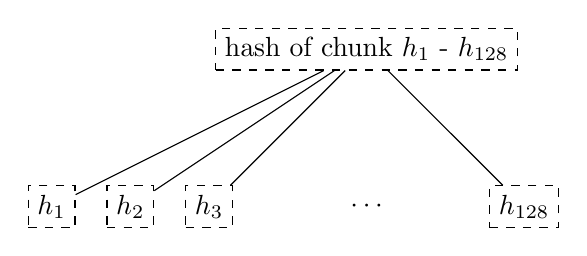
\begin{tikzpicture}
\node[draw,dashed] (root) at (5,3) {hash of chunk $h_1$ - $h_{128}$};
\node[draw,dashed] (h1) at (1,1) {$h_1$};
\node[draw,dashed] (h2) at (2,1) {$h_2$};
\node[draw,dashed] (h3) at (3,1) {$h_3$};
\node (dots) at (5,1) {$\cdots$};
\node[draw,dashed] (h128) at (7,1) {$h_{128}$};
% \node[draw,fit=(h1) (h2) (h3) (dots) (h128)]{};
\draw (root) -- (h1);
\draw (root) -- (h2);
\draw (root) -- (h3);
\draw (root) -- (h128);
\end{tikzpicture}
   \caption{ A generic node in the tree has 128 children.}
   \label{fig:swarm-hash-basic}
\end{figure}

During normal swarm lookups, a swarm client performs a lookup for a hash value and receives a chunk in return. This chunk in turn constitutes another $b$ hashes to be looked up and retrieve another $b$ chunks and so on until the chunks received belong to the actual document (see figure \ref{fig:swarm-hash-split}).


\begin{figure}[htbp]
   \centering
   
\begin{tikzpicture}
\node[draw,dashed] (root) at (5,3) {root hash};
\node[draw,dashed] (h1) at (1,1) {$h_1$};
\node[draw,dashed] (h2) at (2,1) {$h_2$};
\node[draw,dashed] (h3) at (3,1) {$h_3$};
\node (dots) at (5,1) {$\cdots$};
\node[draw,dashed] (h128) at (7,1) {$h_{128}$};
\node[draw,fit=(h1) (h2) (h3) (dots) (h128)]{};
\draw (root) -- (h1);
\draw (root) -- (h2);
\draw (root) -- (h3);
\draw (root) -- (h128);
\node[draw,dashed] (g1) at (-1.4,-1) {$h^1_1$};
\node[draw,dashed] (g2) at (-0.6,-1) {$h^1_2$};
\node (gdots) at (0,-1) {$\cdots$};
\node[draw,dashed] (g128) at (0.7,-1) {$h^1_{128}$};
\node[draw,fit=(g1)(g2)(gdots)(g128)]{};
\draw (h1) -- (g1);
\draw (h1) -- (g2);
\draw (h1) -- (g128);
\node[draw,dashed] (f1) at (1.8,-1) {$h^2_1$};
\node[draw,dashed] (f2) at (2.6,-1) {$h^2_2$};
\node (fdots) at (3.2,-1) {$\cdots$};
\node[draw,dashed] (f128) at (3.9,-1) {$h^2_{128}$};
\node[draw,fit=(f1)(f2)(fdots)(f128)]{};
\draw (h2) -- (f1);
\draw (h2) -- (f2);
\draw (h2) -- (f128);
\node (moredots) at (5,-1) {$\cdots$};
\node[draw] (c1) at (-2.3,-3) {chunk 1};
\node[draw] (c2) at (0,-3) {chunk 2};
\node at (1.4,-3) {$\cdots$};
\node[draw] (c129) at (3,-3) {chunk 129};
\node (cdots) at (4.5,-3) {$\cdots$};
\node[draw] (cn) at (6,-3) {chunk N};
\draw (g1) -- (c1);
\draw (g2) -- (c2);
\draw (f1) -- (c129);
\end{tikzpicture}
   \caption{ The swarm tree is the data structure encoding how a document is split into chunks.}
   \label{fig:swarm-hash-split}
\end{figure}

While off-the-shelf erasure coding could be used on documents uploaded in swarm, this solution has immediate problems. Apart from the quadratic complexity of encoding, chunking the CRS-encoded datablob with the chunker would result in certain chunks being more vulnerable, since their retrieval is dependent on the retrieval of the chunks that encode all their ancestor nodes in the chunktree.

This prompted us to try and align the notion of swarm chunk with the chunk used in the CRS scheme. This led us to encode redundancy directly into the swarm tree by applying the \emph{CRS scheme}  to each set of chunks that are children of a node in the swarm tree.

The \emph{chunker} algorithm using CRS coding works the following way when splitting the document:

\begin{enumerate}
\item Set input to the data blob.
\item Read the input one chunk (say fixed 4096 bytes) at a time. Count the chunks by incrementing a counter $i$. 
\item Repeat 2 until either there's no more data (note: the last chunk read may be shorter) or $i \equiv 0$ mod $m$
\item use the CRS scheme on the last $i \mod\ m$ chunks to produce $k$ parity chunks resulting in a total of $n \leq m+k$ chunks.
\item Calculate the hashes of all these chunks and concatenate them to result in the next chunk (of size $i\mod m$ of the next level. Record this chunk as the next.
\item If there is more data repeat 2. 
\item If there is no more data but the next level data blob has more than one chunk, set the input to this and repeat from 2.
\item Otherwise remember the blob as the root chunk.
\end{enumerate}

% Fixing the branching factor of the swarm hash as $n=128$ and $h=32$ as the size of the \emph{SHA3 Keccak hash} gives us a chunk size of $4096$ bytes.

% We start splitting the input data into chunks, and after each $m$ chunks add $k=n-m$ parity check chunks using a Reed-Solomon code so that now any $m\text{-out-of-}n$ chunks are
% sufficient to reconstruct the document. On the next level up the chunks are composed of the hashes of the $m$  data chunks and the $k$ hashes of the parity chunks. Let's take the first $m$
% of these and add an additional $k$ parity chunks to those such that any $m$ of the resulting $n$
% chunks are sufficient to reconstruct the origial $m$ chunks. And so on and on every level. In terms of
% availability, every subtree is equally important to every other subtree at this level. The resulting
% data structure is not a balanced tree since on every level $i$ the last $k$ chunks are parity leaf
% chunks while the first $m$ are branching nodes encoding a subtree of depth $i-1$ redundantly.
A typical piece of our tree would look like this (see figure \ref{fig:swarm-hash-erasure}).


\begin{figure}[htbp]
   \centering
   \begin{tikzpicture}[
level/.style={sibling distance=15mm, line width=0.6pt, level distance=18mm},
hash/.style={fill=white, rounded corners=2pt,draw,minimum size=1.2cm},
phash/.style={fill=lightgray!50, rounded corners=2pt,dotted,draw,minimum size=1.2cm},
chunk/.style={fill=lightgray, rounded corners=2pt,draw,minimum size=1.2cm},
midchunk/.style={draw=none,minimum size=0.2cm}
]

% root node
\node [hash] (root) {$H$}
  % vertical arrow
  child[grow=down,draw=none] { node {} edge from parent[<-,shorten >=12pt]}
  % annotation
  child[grow=right,draw=none,level distance=5cm] { node (swh) {Swarm root hash} edge from parent[draw=none] }
  % level n
  child {node [hash] (n-10) {$H_{0}$} edge from parent[draw=none]
    % arrow
    child[grow=down,draw=none] { node {} edge from parent[<-, shorten >=12pt]}
    % annotation
    % child[grow=left,draw=none,level distance=4cm] { node[align=center] at (-4,1) (bnl) {intermediate\\branching nodes\\chunks of 128 hashes}  edge from parent[draw=none] }
    % level n-1
    child {node [hash] (n-2l0) {$H_{0}$} edge from parent[draw=none]
      % level 2 compressed
      child[thick] {node [midchunk] (2l0) {} edge from parent[draw=none]
        % level 1
        child {node [hash] at (0,1.2) (1l0) {$H_{0}$} edge from parent[draw=none]
          % level 0
          child[grow=down,draw=none] { node {} edge from parent[<-, shorten >=12pt]}
          child {node [hash] (0l0) {$H_{0}$} edge from parent[<-, draw=none]
            child {node [chunk] {$C_{0}$}}
          }
          child {node [hash] (0l1) {$H_{1}$} edge from parent[<-, draw=none]
            child {node [chunk] (cl1) {$C_{1}$}}
          }
          child[missing]
          child {node [hash] (0ll) {$H_{111}$} edge from parent[<-, draw=none]
            child {node [chunk] (cll) {}}
          }
          child { node [phash] (p1-0ll) {$P_{0}$} edge from parent[draw=none]}
          child[missing]
          child { node [phash] (p15-0ll) {$P_{15}$} edge from parent[draw=none]}
        }
        % level 1 siblings
        child {node [hash] at (0,1.2) (1l1) {$H_{1}$} edge from parent[draw=none]
          child[thick,loosely dotted, shorten >=6mm, thick,<-] {node {}}
        }
        child[missing]
        child {node [hash] at (0,1.2) (1ll) {$H_{111}$} edge from parent[draw=none]
          child[thick,loosely dotted, shorten >=6mm, thick,<-] {node {}}
        }
        child { node [phash] at (0.2,1.2) (p1l) {$P_{0}$} edge from parent[draw=none]}
        child[missing]
        child { node [phash] at (0,1.2) (p1l0) {$P_{15}$} edge from parent[draw=none]}
      }
    }
    % level n-1 siblings lhs
    child {node [hash] (n-2l1) {$H_{1}$} edge from parent[draw=none]
      child[thick,loosely dotted, shorten >=6mm, thick,<-] {node {}}
    }
    child[missing]
    child {node [hash] (n-2ll) {$H_{111}$} edge from parent[draw=none]
      child[thick,loosely dotted, shorten >=6mm, thick,<-] {node {}}
    }
    child { node [phash] at (0.2,0) (p1-2ll) {$P_{0}$} edge from parent[draw=none]}
    child[missing]
    child { node [phash] (p15n-2ll) {$P_{15}$} edge from parent[draw=none]}
    child[missing]
    child[missing]
  }
  % level n siblings
  child {node [hash] (n-11) {$H_{1}$} edge from parent[draw=none]
    child[thick,loosely dotted, shorten >=6mm, thick,<-] {node {}}
  }
  child[missing]
  child[missing]
  child[missing]
  child[missing]
  child { node [hash] (n-1l) {$H_{111}$} edge from parent[draw=none]
    % level n-2 siblings rhs vertical arrow
    child[grow=down,draw=none] { node {} edge from parent[<-, shorten >=12pt]}
    % child[grow=right,level distance=9cm] { node[align=center] (bnr)   {intermediate\\branching nodes\\chunks of 128 hashes}edge from parent[draw=none]}
    child[missing]
    child {node [hash] (n-2r0) {$H_{0}$} edge from parent[draw=none]
      child[thick,loosely dotted, shorten >=6mm, thick,<-] {node {}}
    }
    child {node [hash] (n-2r1) {$H_{1}$} edge from parent[draw=none]
      child[thick,loosely dotted, shorten >=6mm, thick,<-] {node {}}
    }
    child[missing]
    child {node [hash] (n-2rl) {$H_{111}$} edge from parent[draw=none]
      % level 2 siblings compressed
      child[grow=down] {node [midchunk] (2rl) {} edge from parent[draw=none]
        % level 1 siblings moved up
        child {node [hash] at (0,1.2) (1r0) {$H_{0}$} edge from parent[draw=none]
          child[thick,loosely dotted, shorten >=6mm, thick,<-] {node {}}
        }
        child {node [hash] at (0,1.2) (1r1) {$H_{1}$} edge from parent[draw=none]
          child[thick,loosely dotted, shorten >=6mm, thick,<-] {node {}}
        }
        child[missing]
        child {node [hash] at (0,1.2) (1rl) {$H_{111}$} edge from parent[draw=none]
          % level 0 siblings rhs
          child[grow=down,draw=none] { node {} edge from parent[<-, shorten >=12pt]}
          child {node [hash] (0r0) {$H_{0}$} edge from parent[<-, draw=none]
            child {node [chunk] (cr0) {}}
          }
          child {node [hash] (0r1) {$H_{1}$} edge from parent[<-, draw=none]
            child {node [chunk] (cr1) {}}
          }
          child[missing]
          child {node [hash] (0rl) {$H_{111}$} edge from parent[<-, draw=none]
            child {node [chunk] (crl) {$C_{m}$}
            %   child [grow=right] { edge from parent[draw=none]
            %     child [grow=right] {node[align=center] {leaf chunks\\data level} edge  from parent[draw=none]
            %       child [grow=up] {node {level $0$} edge from parent[draw=none]
            %         child [grow=up] {node {level $1$} edge from parent[draw=none]
            %             child [grow=up] {node at (0,0.8) {level $n-1$} edge from  parent[draw=none]
            %               child [grow=up] {node {root = level $n$} edge from  parent[draw=none]}
            %             }
            %         }
            %       }
            %     }
            %   }
            }
          }
          child { node [phash] at (0.2,0) (p100) {$P_{0}$} edge from parent[draw=none]}
          child[missing]
          child { node [phash] (p150) {$P_{15}$} edge from parent[draw=none]}
        }
        child { node [phash] at (0.2,1.2) (p11) {$P_{0}$} edge from parent[draw=none]}
        child[missing]
        child { node [phash] at (0,1.2) (p151) {$P_{15}$} edge from parent[draw=none]}
      }
    }
    child { node [phash] at (0.2,0) (p1n-2) {$P_{0}$} edge from parent[draw=none]}
    child[missing]
    child { node [phash] (p15n-2) {$P_{15}$} edge from parent[draw=none]}
  }
  child { node [phash] at (0.2,0) (p1n) {$P_{0}$} edge from parent[draw=none]}
  child[missing]
  child { node [phash] (p15n-11) {$P_{15}$} edge from parent[draw=none]};

% elipsis
\path (p1n) -- (p15n-11) node [midway,font=\large] {$\ldots$};
\path (p1n-2) -- (p15n-2) node [midway,font=\large] {$\ldots$};
\path (p11) -- (p151) node [midway,font=\large] {$\ldots$};
\path (p100) -- (p150) node [midway,font=\large] {$\ldots$};
\path (p1l) -- (p1l0) node [midway,font=\large] {$\ldots$};
\path (p1-0ll) -- (p15-0ll) node [midway,font=\large] {$\ldots$};
\path (p1-2ll) -- (p15n-2ll) node [midway,font=\large] {$\ldots$};


\path (n-11) -- (n-1l) node [midway,font=\large] {$\ldots$};
\path (n-2l0) -- (2l0) node [midway,font=\large,sloped] {$\ldots$};
\path (n-2rl) -- (2rl) node [midway,font=\large,sloped] {$\ldots$};
\path (1l1) -- (1ll) node [midway,font=\large] {$\ldots$};
\path (1r1) -- (1rl) node [midway,font=\large] {$\ldots$};
\path (p1l0) -- (1r0) node [midway,font=\large] {$\ldots$};
\path (n-2l1) -- (n-2ll) node [midway,font=\large] {$\ldots$};
\path (n-2r1) -- (n-2rl) node [midway,font=\large] {$\ldots$};
% \path (n-2ll) -- (n-2r0) node [midway,font=\large,sloped] {$\ldots$};
\path (0l1) -- (0ll) node [midway,font=\large] {$\ldots$};
\path (0r1) -- (0rl) node [midway,font=\large] {$\ldots$};
% \path (0ll) -- (0r0) node [midway,font=\large] {$\ldots$};
% \path (cl1) -- (cll) node [midway,font=\large] {$\ldots$};
% \path (cr1) -- (crl) node [midway,font=\large] {$\ldots$};
% \path (cll) -- (cr0) node [midway,font=\large] {$\ldots$};
% \path (p1) -- (p15) node [midway,font=\large] {$\ldots$};


% arrows from annotations
\begin{scope}[shorten >=.5cm,thin]
\draw [->] (swh) -> (root);
% \draw [->] (bnl) -> (n-10);
% \draw [->] (bnl) -> (n-2l0);
% \draw [->] (bnl) -> (1l0);
% \draw [->] (bnl) -> (0l0);
% \draw [->] (bnr) -> (n-1l);
% \draw [->] (bnr) -> (n-2rl);
% \draw [->] (bnr) -> (1rl);
% \draw [->] (bnr) -> (0rl);
\end{scope}

% boxes to group nodes
% \node[rounded corners=2pt, draw=white, minimum height=1.1cm, fit=(root)] {};
\node[rounded corners=2pt, draw=black, minimum height=1.1cm, fit=(n-10) (p15n-11)] {};

\node[rounded corners=2pt, draw=black, minimum height=1.1cm, fit=(0l0) (p15-0ll)] {};
\node[rounded corners=2pt, draw=black, minimum height=1.1cm, fit=(n-2l0) (p15n-2ll)] {};
\node[rounded corners=2pt, draw=black, minimum height=1.1cm, fit=(n-2r0) (p15n-2)] {};
\node[rounded corners=2pt, draw=black, minimum height=1.1cm, fit=(1l0) (p1l0)] {};
\node[rounded corners=2pt, draw=black, minimum height=1.1cm, fit=(1r0) (p151)] {};

\node[rounded corners=2pt, draw=black, minimum height=1.1cm, fit=(0r0) (p150)] {};

\end{tikzpicture}
   \caption{The swarm tree with extra parity chunks using $m$ out of 128 CRS code. Chunks $p^{m+1}$ through $p^{128}$ are parity data for chunks $h^1_1 - h^1_{128}$ through $h^{m}_1  - h^{m}_{128}$.}
   \label{fig:swarm-hash-erasure}
\end{figure}


This pattern repeats itself all the way down the tree. Thus hashes $h^1_{m+1}$ through $h^1_{128}$ point to parity data for chunks pointed to by $h^1_1$ through $h^1_{m}$. Parity chunks $p^i$f do not have children and so the tree structure does not have uniform depth.

\subsubsection{Incomplete batches}

If the number of file chunks is not divisible by $m$, we cannot proceed with the last batch in the same way as the others. We propose that we encode the remaining chunks with an erasure code that guarantees at least the same level of security as the others. Note that it is not as simple as choosing the same redundancy. For example a 50-of-100 encoding is much more secure against loss than a 1-of-2 encoding even though the redundancy is 100\% in both cases. Overcompensating, we require the same number of parity chunks even when there are fewer than $m$ data chunks.

This leaves us with only one corner case: it is not possible to use our $m\text{-out-of-}n$ scheme on a single chunk ($m=1$) because it would amount to $k+1$ copies of the same chunk. The problem is that any number of copies of the same chunk all have the same hash and therefore are automatically deduplicated. Whenever a single chunk is left over ($m=1$) (this is always the case for the root chunk itself), we propose to replicate the chunk as the payload of a single-owner chunk with an address that is deterministically derivable from the content owners public key and the original root hash. 

When downloading a file with erasure coding, data subsumed under an intermediate chunk can be recovered having any $m$ out of $m+k$ children. Downloader can initiate requests for all $m+k$ and need to wait  only for the first $m$ to be delivered in order to proceed.  
This technique can effectively shield unavailability of chunks due to occasional faults like network contention, connectivity gaps, and node churn; prohibitively overpriced neighbourhoods or even attacks targetting certain localities. Given a particular fault model for churn and throughput, erasure codes can be calibrated,
guarantee an upper limit on retrieval latencies, a strong quality proposition.





\subsection{Pinning content}\label{sec:pinning}



    upload with pin header flag
    http interface for bzz-pin for PUT/DELETE for pinning just a hash/ens name
    generalise mechanism for restricting localhost for admin functionality
    cli interface for get/add/delete pins
    traversal for downloading and pinning a hash
    implement reference count in localstore
    manage pinned content volume in connection with overall swarm volume (i.e. should not interfere with storage for regular purposes)
    feed content pinning

\subsection{Re-upload and missing chunk notifications}\label{sec:reupload}

 when a content is pinned on a Swarm node, it is guaranteed to be available on that local node ONLY. When the same content is retrieved from another Swarm node, it uses the 'network copy'. If the network copy of the particular pinned content disappears as a result of garbage collection, pinning itself offers no way to retrieve this content. in order to utilise pinning in aiding persistence, a few issues need to be addressed.

In part 2 of pinning, this drawback needs to be addressed. i.e. pinned contents should be available from any Swarm node.


    A way for other swarm nodes to locate the pinned Swarm node for a given pinned content

    Pinning servers should advertise their PSS address so that other Swarm nodes that need the content, can contact the pinned Swarm node to retrieve the contents they hold. One way to do this is to add the PSS address of the pinning node to the manifest of the contents when they are uploaded and pinned. The best way to do this is to have the reference to a pinning feed included in the manifest.

    Respective Pinned nodes to get indication of their pinned contents disappearing from the network.

    [Method-1] One naive way to achieve this is to periodically check for random pinned chunk in the network and re-upload the contents if they are not found.

    [Method -2] Another way is, When someone access the pinned contents from another Swarm node and if it finds that the content is not available in the network, then it notifies the pinning node(s) by updating a pinning feed.

    Re-upload the pinned contents in to the Swarm network

    Once the pinning node(s) received a notification that the pinned contents are missing from the network, they re-sync the contents to the Swarm network as if they are uploaded just now.

Optimizations that can be done later

    Stream the contents from the pinned node to the requesting node

Once dis-advantage of point 3, is that the requesting Swarm node hash to wait for the contents to be re-synced to the network and then start downloading them. The issue with this is identify when exactly all the contents are synced in the network to start downloading.

One way to avoid this dilemma, is to have a streaming sync protocol between the pinned node and the downloading Swarm node so that the pinned contents can be shared directly. Ofcourse, this method has some load considerations and should be multi-routed to avoid single path.

    Pinned nodes to upload only the GC'd chunks to the network

When the pinned node gets an indication that the content has disappeared from the network, it is not necessary that the entire pinned directory or file is missing. Few chunks of the pinned content may be sparsely used and it is possible that only they are GC'd. So instead of re-syncing all thechunks of the pinned content, pinning servers can somehow find what chunks are missing and re-sync only them to avoid unnecessary sync load on the network.
Context

When a user uses a pinning service and pins hs contents (a website for example), he should be able to access his pinned contents from any Swarm node. This helps in more de-centralisation of contents access.

\subsection{Insurance}\label{sec:insurance}


\section{Access control}\label{sec:access-control}

The encryption described in the previous section becomes useful once the users are provided a way to manage access to the decryption key, ie., full reference to restricted content.  
Usecases include managing private shared content as well as authorising access to member's areas of web applications, traditionally handled by login and centralised gate-keeping.

\subsection{Encryption}\label{sec:encryption}

This section describes how to achieve confidentiality in a  public storage like swarm. 
It is a natural requirement for many use cases to store private information accessible only to authorized parties in Swarm. 

It is clear that pseudo-confidentiality by server-based access  control predominantly used in current web applications is inadequate. In Swarm nodes are expected to share the chunks with other nodes, in fact, storers of chunks are  incentivised to serve them to requestors, therefore it is unlikely that nodes can be as gatekeepers trusted with controlling access. Moreover, since every node could potentially be a storer, the confidentiality solution must leak nothing that helps 3rd party storers to distinguish a private chunk from random data. As a consequence, the only way to prevent unauthorized parties from accessing private chunks is encryption. In swarm, if a requestor is authorized to access a chunk, they must be in possession of decryption key to be used to decrypt the chunk, while unauthorized parties must not. Incidentally this also serves as the basis for \gloss{plausible deniability}.

Encryption on the chunk level as described in \ref{sec:chunk-encryption} and formally specified in \ref{spec:format:chunk-encryption}
has the desireable property that it is virtually independent of the chunk store layer, with the exact same underlying infrastructure for storing and retrieving chunks as the case of unencrypted content.
The only difference between accessing private and public data is the presence of a decryption/encryption key in the chunk references (see \ref{spec:format:files}) the computational overhead related to encryption, a constant or linear factor.

The storage API raw GET entrypoint allows both encrypted and unencrypted chunk  references. 
Decryption is  triggered if the chunk reference is double size; consisting of a ciphertext hash and a decryption key.  It retrieves the ciphertext chunk from the chunk,  stores and decrypts it using the supplied decryption key, and returns the plaintext chunk.

The chunk store API post endpoint expects users to indicate if they want to have encryption on the upload or not. In both cases the chunk will be stored and push-synced to the network, but if encryption is desired the ciphertext chunk needs to be created first. If no further context is given, a random encryption key is generated, which is used as seed to generate random padding to fill the chunk to a complete 4096 bytes if needed and finally this plaintext is encrypted with the key. In case of encryption the API post call returns both the Swarm hash and the encryption key constituting the swarm reference. 

In order to guarantee the uniqueness of encryption keys as well as to ease the load on the OS's entropy pool, it is recommended (but not required) to generate the key as the MAC of the plaintext using a (semi-) permanent random key stored in memory. 
This key can be permanent and generated using scrypt with a password supplied upon startup. Instead   of the plaintext, a namespace and path of the manifest entry can be used as context.
This has the consequence that chunk encryption is deterministic as long as the context is the same: if we exchange one byte of a file and encrypt it with the same context, all data chunks of the file but the one actually modified will end up being encrypted exactly as the original (see \ref{spec:format:encryption}). Encryption is therefore deduplication friendly. 


\subsection{Managing access}\label{sec:managing-access}

This section describes the process the client needs to follow in order to obtain full reference to encrypted content. This protocol needs basic meta-information which is encoded as plaintext metadata and explicitly included in the root manifest entry for a document. This non-priviliged access is called \gloss{root access}.

In contrast, \gloss{granted access} is a type of selective access requiring root access as well as access credentials: authorized private key or passphrase. Granted access gives differentiated privileges accessing the content to multiple parties sharing the same root access. This allows for updating the content without changing access credentials. Granted access is implemented by an additional layer of encryption on references.

The symmetric encryption of the reference is called \gloss{encrypted reference}, the symmetric key used in this layer is called
\gloss{access key}.

In case of granted access, the root access meta-information contains both the encrypted reference and additional information for obtaining the access key using access credentials. Once the access key is obtained, the reference to content is obtained by decrypting the encrypted reference with the access key resulting in the full reference composed of the address root chunk and the decryption key for the root chunk. 

The access key can be obtained from a variety of sources, of which currently three are defined.

First, a \gloss{session key} is derived from the provided credentials. In case of granting access to a single party, the session key is used directly as the access key. In case of multiple parties, an additional mechanism is used for turning the session key into the access key.

\subsubsection{Passphrase}
The simplest credential is a \emph{passhrase}. The session key is derived from a passphrase using 'scrypt' with parameters specified among the root access meta-information. The output of `scrypt` is a 32-byte key that can be directly used for Swarm encryption and decryption algorithms.

In typical use cases, the passphrase is distributed by off-band means with adequate security measures. Any user knowing the passphrase from which the key was derived can access the content.

\subsubsection{Asymmetric derivation}

A more sophisticated credential is a \emph{private key}, identical to those used throughout Ethereum for accessing accounts, i.e., elliptic curve using secp256k. In order to obtain the session key, an ECDH key agreement needs to be performed between the content publisher and the grantee. The resulting shared secret is hashed together with a salt. The content publisher's public key as well as the salt are included among metadata in the root access manifest. It follows from the standard assumptions of ECDH, that this session key can only be computed by the publisher and the grantee and noone else (by ECDH assumption). 
Once again, if access is granted to a single public key, the session key derived this way can be directly used as the access key which allows decrypting the encrypted reference. 

\subsection{Selective access to multiple parties}

In order to manage access by multiple parties to the same content, an additional layer is introduced to obtain the access key from the session key. In this variant, grantees can be identified by either type of credentials, however the session key derived as
described above is not used directly as access key to decrypt the reference. Instead, two keys, a \gloss{lookup key} and a \gloss{access key decryption key} are derived from it by hashing it with two different constants (1 and 0, respectively).

When granting access, the publisher needs to generate a global access key to encrypt the full reference and encrypt it with the
access key decryption keys for each grantee. Thereafter, they need to create a lookup table mapping grantees' lookup keys to the encrypted access key. For each lookup key, the access key is encrypted with the corresponding access key decryption key.

This lookup table is implemented as an \gloss{access control trie} (a.k.a. ACT) in Swarm manifest format with paths corresponding to lookup keys and manifest entries containing the ciphertext of the encrypted access keys as metadata attribute value. The ACT manifest an independent resource referenced by a URL included among the root access metadata so that users know whether to use ACT.

When accessing content, the user retrieves the root access meta data, identifies the ACT resource, calculates their session key (using their passphrase and the scrypt parameters or the publisher public key and their private key and a salt). From the session key they derive the lookup key by hashing it with 0, they then retrieve the manifest entry from ACT. For this they need to know the root of the ACT manifest and the use the lookup key for the URL path. If the entry exists the user takes the value of the access key attribute. This is a ciphertext that is decrypted with a key derived by hashing the session key with constant 1. The resulting access key can then be used to decrypt the encrypted reference included in the root access manifest.

This access control scheme has a number of desireable properties:
\begin{itemize}
\item Checking and looking up one's own access is logarithmic in the size of the ACT.
\item The size of the ACT merely provides an upper bound on the number of grantees, but does not disclose any information beyond this upper bound about the set of grantees to third parties. Even those included in the ACT can only learn that they are grantees, but obtain no information about other grantees beyond an upper bound on their number.
\item Granting access to an additional key requires extending the ACT by a single entry, which is logarithmic in the size of the ACT. 
\item Withdrawing access requires a change in the access key and therefore the rebuilding of the ACT. Note that this requires that the publisher keeps the public keys of grantees after the initial ACT is created.
\end{itemize}

\subsection{Access hierarchy}

In the simplest case, the access key is a symmetric key. However, this is just a special case of the more flexible solution, where
the access key consists of a symmetric key and a key derivation path by which it is derived from a root key. In this case, in addition to the encrypted reference, a derivation path may also be included. Any party with an access key whose derivation is a prefix to the derivation path of the reference can decrypt the reference by deriving its key using their own key and the rest of the derivation path of the reference.

This allows for a tree-like hierarchy of roles, possibly reflecting an organizational structure. As long as role changes are "promotions", i.e. result in increase of privileges, it is sufficient to change a single ACT entry for each role change.

The exact format of manifests as well as the serialisation conventions are specified in more detail in \ref{spec:format:access-control}

\section{User interface for storage}\label{sec:storage-ux}

\subsection{Upload}\label{sec:upload}


\subsubsection{Postage}

To impose a cost on uploads and efficiently allocate storage resources in the network, all uploads must be paid for.  This is somewhat unusual for the web, so a novel user experience needs to be developed. The closest and most familiar metaphor is a subscription.

The user creates a subscription for a certain amount of time and storage (e.g. 1 month for 100 megabytes) and pays for it, according to a price they learn from the client software (similar to transaction fees on the blockchain). Subscriptions are named, but these names are only meaningful locally.

When the user uploads files, they also indicate which subscription to use, or the most recent one is used as default.

When checking their subscription(s), the user is informed how much data has already been uploaded to that subscription and how much can be stored given the current price (e.g. 88/100 megabytes). Note that the second part can also change, if the prices change (e.g. 88/90).

If the first part is more than the second part (95/90), it means that uploaded content is in danger of being garbage collected and therefore to prevent that topping up their subscription is instructive.

\subsubsection{Tags and progress bar}

\subsubsection{Resuming uploads}
\subsubsection{Encryption}
\subsubsection{Pinning}
\subsubsection{Erasure coding}

\subsection{Manipulating manifests}\label{sec:manifests-ux}

\subsubsection{Updating collections} 

\subsubsection{Controlling access}



\subsection{Download}\label{sec:upload}


\chapter{Communication}\label{sec:messaging}

Somewhat surprisingly, swarm's network layer can serve as  an efficient  communication platform with exceptionally strong privacy properties. This chapter is an attempt to define a comprehensive set of primitives that serve as building blocks for a base layer communication infrastructure covering the full range of communication modalities including real time anonymous chat, sending and receiving messages from previously not connected, potentially anonymous senders, mailboxing for asynchronous delivery, long term notifications and  publish/subscribe interfaces. 


First, in \ref{sec:feeds}, we introduce swarm feeds, which are suitable for representing a wide variety of sequential data, such as versioning updates of a mutable resource or indexing messages for real-time data exchange offering a system of persisted pull messaging. To implement push-notifications of all kinds, \ref{sec:pss} introduces trojan chunks that allow messages to be disguised as chunks and also show how to direct them to a recipient. Finally, \ref{sec:comms-ux} describes a high-level communication API. 


% \section{Derivative resources}


% \begin{equation}
%     \mathit{Addr}(x)\defeq\mathit{Hash}(\mathit{Pub}(x)|\mathit{Hash}(\mathit{par}|\mathit{rel}|\mathit{seq}))
% \end{equation}
% where 
% \begin{itemize}
%     \item[$par$] is the content address of the parent resource
%     \item[$rel$] is the content address of the derivative relation type (e.g., comment, evaluation, sequel, revision, part)
%     \item[$seq$] is the sequence position (an incrementing counter starting with 0) 
% \end{itemize}


\section{Swarm feeds and mutable resource updates}\label{sec:feeds}

Assoc chunks are the basis of swarm feeds. A feed chunk is an assoc chunk with the associated constraint that the identifier is composed as the hash of a \emph{topic} and an \emph{index}. 

\subsection{Using feeds for versioning}\label{sec:feed-as-channel}

Feeds are used for versioning revisions of a mutable resource, indexing sequential updates to a topic, publish the parts to infinite streams, or post consecutive messages in a communication channel. Feeds implement persisted pull-messaging and can also be interpreted as a pub-sub system. Publishers are the single owners of feed chunks and are able to post updates to the feed by constructing the address of an assoc chunk and signing arbitrary content to it. Conversely, consumers can subscribe to updates of a feed by a publisher they know by constructing the address for the request which only requires the user to know the identifier and the publisher address to look up the content. 

\subsection{Timestamp based feeds}\label{sec:time-based-feeds}

\subsection{Integrity}\label{sec:feed-integrity}

Publishers can commit to the integrity of their feeds by staking a deposit on the blockchain they stand to  lose if they double sign on an update.%
%
\footnote{Single-owner chunks can also be used to provide soft consensus. We illustrate this with an example of off-chain payments where  consensus  is needed on funds allocation over a fixed set of creditors. If a debitor keeps publishing a deposit allocation table for an exhaustive list of creditors, by issuing two alternatives to targeted creditors the debitors can orchestrate a double spend. Conversely, certainty in the uniqueness of the allocation table allows the creditor to conclude finality. In the case of deposit increase, the creditor checks the reallocations, i.e., the total increases are covered by countersigned decreases. See more  detail in \cite{tronetal-sw3games}.)}
%
Such feeds with enforced integrity can be used as an authoritive audit trail of a mutable resource.%
%
\footnote{If the chunks are uploaded using the same route, the chunk that comes later will be rejected as already known. If the two chunks originate from different addresses in the network, they might both end up in their local neighbourhood. This scenario will result in inconsistent retrievals depending on which node the request ends up with.}
%
The most important property is that it is impossible to meaningfully control the responses to a single-owner chunk request. In particular there is no systematic way to respond with particular versions to particular requestors even if we control the neighbourhood of the chunk  address. This is the result of anonymous retrievals enabled by forwarding kademlia. In fact by sending several requests from random addresses, a requestor can be sure of the uniqueness of the payload with any desired degree of certainty. 
As a consequence, publishers are not expected to create single-owner chunk collisions, since consumers are able to detect it.  



\subsection{Real-time data exchange}\label{sec:real-time-data-exchange}

As long as the public key and the naming conventions are known to some users, they can follow updates. If two parties mutually follow one another's outbox feed, it effectively results in a bidirectional communications channel. If several parties know each others keys and follow each other's outbox, one can implement group messaging or forums. 

% \section{Feeds used in realtime exchange}\label{sec:feeds-for-comms}

The outbox-based solution presented above has its limitations. It assumes that the communicating parties know each others public keys. There are genuine use cases when permissionless first time contact with a public identity is required. In other words, there needs to be a way for a party unknown to the recipient to initiate communication. Since such a solution makes unsolicited contact possible, spam protection measures should be in place.

Channel communication is smooth in the case of real-time interaction, when outboxes are queried (or at worst polled). If the communication channel has irregular asynchronicities, i.e., updates can have unpredictable gaps, polling is suboptimal as it generates a lot of bandwidth overhead. There needs to be a way for a sender to notify recipient of an update, i.e., restart communication in a channel. Conversely, there needs to be a way for the recipient to be notified  about the  sender's activity on a channel. This is more relevant in case of public feeds where consumers are not necessarily known to the publisher. 

We distinguish two cases here: one use case is when the recipient/consumer watches a feed/outbox and waits for the next update which is not guaranteed to come at regular interval, so consumer wants to save on polling. The other case is when there is a feed with irregular updates and the consumer is assumed to have missed an arbitrary number of updates.
In such a case timestamp based indexing is needed with a logartithmic search.

In the case of many to many group channels (forums), polling is suboptimal as it requires each user to poll a large number of outboxes, while other participants do the same. In such cases aggregation of feeds into indexes is required which can then be polled or subscribed to by individual users.

To sum up:

\begin{itemize}
    \item \emph{start a new channel} - permissionless contact           
    \item \emph{restart a channel} - contact after arbitrary period
    \item \emph{subscribe to a channel} - notification of updates without polling
    \item \emph{find the latest update} - efficient search for the latest update in a channel
    \item \emph{aggregate updates} - efficient way to get updates from a large number of updates to a multiparty channel
\end{itemize} 

\section{Direct push messaging with}\label{sec:pss}

\subsection{Trojan chunks}\label{sec:trojan}

Cutting edge systems promising private messaging often struggle to offer truly zero leak communication. While linking of sender and recipient is cryptographically proven to be impossible, resistance to traffic analysis is harder to achieve. Having sufficiently large anonimity sets requires high volumes available at all times. In the absence of mass adoption, guaranteeing high traffic in dedicated messaging networks necessitates constant fake traffic. 

With swarm, the opportunity arises to disguise messaging as chunk traffic and thereby obfuscate the act of messaging. We define a \gloss{trojan} chunk as a content addressed chunk with a fixed structure:

\begin{enumerate}
    \item \emph{nonce} - 32 byte arbitrary nonce 
    \item \emph{trojan  message} - 4000 byte asymmetrically encrypted message ciphertext with underlying plaintext composed of
    \begin{enumerate}
        \item \emph{length} - 2 byte bigendian encoding of length of message in bytes $0\leq l\leq 3968$
        \item \emph{integrity protection} the last 30 bytes of the hash of the payload 
        \item \emph{payload} - $l$ bytes of message that is the serialisation of a swarm message
        \item \emph{padding} - $4000-l-32$ random bytes
    \end{enumerate}
\end{enumerate}

Knowing the public key of the recipient, sender encrypts the message (after prefixing it with its length and padding it) using asymmetric encryption. Then sender tries to find a random nonce so that when prepended to the payload, it hashes to an address that falls in the neighbourhood of the recipient based on the overlay address derived from the public key%
%
\footnote{Alternative overlays can be associated with a public key, and several public keys can be listened on by a node at a particular address.}
%
(see \ref{spec:format:bzzaddress}). The sender then uploads the resulting chunk to swarm with postage stamps of their choice which then ends up being synced to the recipient address' neighbourhood. If the recipient node is online they receive the chunk for certain if they are the closest node. 

\subsubsection{Receiving trojan messages}

The recipient knows that a chunk is such a trojan message if and when they try to open the message with the private key corresponding to the base account public key and then verify the integrity by hashing the payload and checking the hash against the integrity protection field of the message. 
Nodes that want to receive such trojan messages will keep trying to open all messages that they are closest to.

Note that forwarding nodes (or anyone else apart from sender and recipient) has no way to distinguish between a random encrypted chunk and the trojan, effectively obfuscating the message.  

\subsubsection{Mailboxing for asynchronous delivery}

If the recipient is not online the chunk will prevail as any other chunk would depending on the postage stamp it has. Whenever the recipient node comes online, it pull-syncs from the neighbourhood the chunks closest to it, among them all the trojan chunks. In other words trojan messages automatically provide \emph{mailboxing} functionality, i.e., 
without any further action needed from sender, undelivered messages are preserved and available to the recipient whenever they come online. The duration of mailboxing is controlled with the postage stamps exactly the same way as, in fact, indistinguishable from, the persistence of chunks. 

\subsubsection{Mining difficulty}

The process of finding a hash close to the recipient address is the same as mining blocks on the blockchain, the nonce in the chunk also plays exactly the same role as a block nonce: it provides sufficient entropy to guarantee a solution. The difficulty of mining corresponds to the minimum proximity order required to ensure that the recipient will receive the message and needs to be higher than the neighbourhood depth of the recipient when it comes online, so it is logarithmic in the number of nodes in the network. The expected number of nonces that need to be tried per trojan message before an appropriate content address is found is exponential in the difficulty, and therefore equal to the number of nodes in the network. As the computational cycles needed is on the scale of network size, in practice, mining a trojan 
will never be prohibitively expensive or slow for a single node. The small delay in the second range is expected only at a billion nodes and even that is acceptable given that trojan messages are meant to be only for one-off initiations of a channel. All subsequent real-time exchange will happen using the bidirectional outbox model using single-owner chunks.

\subsection{Addressed envelopes}\label{sec:addressed-envelopes}

The question immediately arises whether it makes sense to somehow mine single-owner chunks. Since the address in this case is the hash of a 32 byte id and a public key, the id provides enough entropy even for a fixed public key to mine arbitrary addresses. Since the address can be mined before the chunk content is associated with it, it can serve as an \emph{addressed envelope}. If we mine an id for a public key so that the resulting single-owner chunk address is close to a target overlay address and we give it to the owner of the corresponding private key, we effectively allow them to send an anonymous message to the target without computation. All they need to do is when they wish to send a message to the target, they create a trojan message and sign it under the premined address. If they sign with the private key corresponding to the public key that is used in the address, the chunk will be valid.
These chunks behave the same way as normal trojan messages, their privacy properties being the same if not somewhat better since issuer/recipient can associate a random public key with which the message is encrypted,  or even use symmetric encryption for speed. If postage stamp is prepaid on the address and given to the sender, they can push-sync the chunk to the target without them needing to pay. Such a construct effectively implements \emph{addressed envelopes with prepaid postage} and serve as base layer solutions for various high-level communication needs: 1) push notifications about an update to subscribers without computational or monetary burden on the publisher 2) free contact vouchers 3) no delay direct message response.  

Issuing a prepaid addressed envelope involves the following process:

\begin{enumerate}
    \item \emph{assume} issuer $I$, prospective sender $S$, and prospective recipient $R$ with public keys $P_I, P_S, P_R$ and overlay addresses $A_I, A_S, A_R$
\item \emph{mine} - $I$ finds a nonce $N_R$ such that when used as an index for single-owner chunk address hashes to $H_R$ which is in the nearest neighbourhood of $A_R$
\item \emph{pay postage} - $I$ signs $H$ to produce a witness for an appropriate postage payment to produce stamp $PS_R$ 
\item \emph{encapsulate} - package $N_R$ and $PS_R$ as the prepaid addressed envelope $E$ 
% and encrypt it with $P_S$ then wrap it as a trojan message
% \item \emph{mine} - find a nonce $N_S$ such that the trojan chunk hashes to $H_S$ which is in the nearest neighbourhood of $A_S$. 
\end{enumerate}

Prospective sender $S$ is assumed to receive a prepaid envelope $E$ and carries out  the following steps:
\begin{enumerate}
    \item \emph{decrypt} message with the private key belonging to $P_S$
    \item \emph{deserialise} unpack and identify $PS_R$ and $N_R$, extract $H_R$ from $PS_R$
    \item \emph{verify} postage stamp $PS_R$ as well as check if $N_R$+$P_S$ hashes to $H_R$ to make sure address belongs to  $S$.
    \item \emph{storage} - store $N_R$, $PS_R$ 
\end{enumerate}

When sender wants to use the envelope to send message $M$ to $R$ (potentially unknown to sender), they 
follow the steps:

\begin{enumerate}
        \item \emph{encrypt} the message content $M$ as payload with $P_R$ and wrap it as a trojan message $T$
        \item \emph{hash} the encrypted trojan message resulting in $H_T$
        \item \emph{sign} $H_T$ using $N_R$ as salt with the private key belonging to $P_S$ producing signature $W$
        \item \emph{encapsulate} nonce $N_R$ as id, the signature $W$ and the trojan message $T$ as payload in a valid single-owner chunk with address $H_R$
        \item \emph{post} the chunk with the valid stamp $PS_R$
\end{enumerate}

When $R$ receives chunk with address $H_R$

\begin{enumerate}
    \item \emph{verify} postage stamp $PS_R$ and validate the chunk as a single-owner chunk with payload $T$.
    \item \emph{decrypt} $T$ with the private key belonging to $P_R$
    \item \emph{deserialise} plaintext as trojan message, identify message payload $M$ and check its integrity with the hash field
    \item \emph{consume} $M$
\end{enumerate}

% \subsubsection{Subscribe to publisher}
If $I$ wants to subscribe $R$ to the next activity on a channel $C$ published by $S$, it needs to give $S$ the prepaid addressed envelope as a trojan message to $A_S$.
If $I=R$, the $I$ subscribe themselves.

\subsection{Update notification requests}\label{sec:update-notification-requests} 

Now consider the use case when a publisher does not want to receive direct messages or send out notifications. Is there a way for consumers to "plant" a notification request at the address of the update directly? The challenge is that (prepaid) addressed envelopes so far required that the sender's public key is known, so that they can produce a valid single-owner chunk for the response. 
In this section, we show another technique which allows for the case when sender has not revealed their overlay or refuse to handle notifications.                                                                                                                                                                                                                                                             
If $I$  wants to subscribe $R$ to a  particular update at address $H_U$ derived from $I_U$ and $P_U$, it takes $I_U$ as a private key $K_U$ and corresponding public key $P_U$. It also chooses a random salt $S_U$ and hashes it with $I_U$ to result in a private key $K_{SU}$ and corresponding public key $P_{SU}$. Then mine a single-owner address $H_{SU}$ for $P_{SU}$ with nonce $N_{SU}$ that is close to the recipient address $A_R$ and prepare it as a prepaid addressed envelope. Package the envelope together with the salt $S_U$, encrypt it with $P_U$ as a trojan message and
package it in a single-owner chunk with index $H(H_U)$. Find a key-pair such that if that is used as publisher the chunk address ($H(H(H_U)^P_N)$) falls in the neighbourhood of $H_U$. This chunk is called \gloss{update notification request} and issuer sends it with a postage stamp so that nodes in the proximity of $H_U$ can store it.

When a node in the proximity of $H_U$ receives the desired update chunk, a single-owner chunk with address $H_U$, it tries to find the update notification request with an index $H(H_U)$ (DB indexing needed). It then takes the payload and decrypts it with the index $I_U$ extracted from the incoming chunk used as a private key. The resulting trojan is verified, its payload is deserialised and postage stamp $PS_R$ and salt $S_U$ are extracted from it. Then the salt is used to derive private key $K_{SU}$ with which the actual notification (the content of the incoming update chunk with index and publisher signature) is signed, then create the valid single-owner chunk with nonce $N_{SU}$ as index, the signature and the actual notification as payload at address $H_{SU}$. The node then sends this chunk, called \gloss{update notification} alongside the postage stamp not knowing anything of the recipient's identity or anything about the channel the update was on.

When $R$ receives the notification chunk at address $H_{SU}$, it validates as a single-owner chunk and the update chunk content is extracted. If valid, save the update chunk and call the handler for channel index $I_U$.
If $I=R$, issuer and recipient are the same, then this is a notification request to issuer as recipient.
Typically, the issuer has requested update at $H_U$, then after time-out, the notification request is created and sent but the database has an open request for $H_U$. When it receives the notification from the node that is in the proximity of $H_U$, the chunk is validated, saved and triggers the handler(s).

\begin{itemize}
    \item originator does not need to know public key of any particular node in the neighbourhood of the update
    \item originator does not need to rely on any node to be online
    \item notifier needs to have both the update chunk as well as the notification to write the notification chunk
    \item mining the key and not the index allows notifiers to look up the notification request based on the index 
    \item notification request is not distinguishable from a random single-owner chunk
    \item forwarding nodes cannot change or interpret the notification 
    \item notifier knows nothing about originator or notified peers
\end{itemize}


% \subsection{Anonymous mailbox} 

% A trojan can serve as anonymous registration, e.g., to a mailbox owner. 

\section{User interface for communication}

\subsection{Pss}\label{sec:pss-ux}
\subsection{Feeds}\label{sec:feeds-ux}
